\documentclass[12pt,a4paper]{article}

\usepackage[utf8]{inputenc}
\usepackage[T1]{fontenc}
\usepackage{geometry}
\geometry{margin=1in}
\usepackage{hyperref}
\usepackage{setspace}
\usepackage{amsmath}
\usepackage{amssymb}
\usepackage{listings}
\usepackage{xcolor}
\usepackage{graphicx}
\usepackage{parskip}
\usepackage{titlesec}
\usepackage{float}
\usepackage{pgfgantt}
\usepackage{xcolor}
\usepackage{colortbl}
\usepackage{array}
\usepackage{longtable}
\newcommand{\sectionbreak}{\clearpage}

\lstset{
    language=C++,
    basicstyle=\setstretch{1}\ttfamily\footnotesize,
    keywordstyle=\color{blue}\bfseries,
    stringstyle=\color{red},
    commentstyle=\color{green!60!black},
    numbers=left,
    numberstyle=\tiny\color{gray},
    stepnumber=1,
    breaklines=true,
    frame=single,
    captionpos=b,
    showstringspaces=false
}

\begin{document}
\onehalfspacing
\definecolor{barblue}{RGB}{70,70,70}

% --- Front Page ---
\begin{titlepage}
    \begin{center}
        \vspace*{1cm}

        \Huge
        \textbf{Market Simulation for Algorithmic Trading}

        \vspace{1cm}

        \Large
        \textbf{by} \\
        \vspace{0.5cm}
        BHANDARI Om Raj \\
        CHOY Ping Hang Gordon \\
        KWONG Wing Fung Josh

        \vspace{1cm}

        \textbf{Advised by} \\
        \vspace{0.5cm}
        Prof. Pedro SANDER

        \vspace{1.5cm}

        \Large
        Submitted in partial fulfillment of the requirements for COMP 4981 \\
        (PSAN4)

        \vspace{0.5cm}

        \Large
        in the \\
        \textbf{Department of Computer Science} \\
        \textbf{The Hong Kong University of Science and Technology}

        \vfill

        \Large
        2025-2026

    \end{center}
\end{titlepage}

\begin{abstract}
This project presents a highly modular, low-latency simulated stock exchange designed for algorithmic trading education. We systematically downscale complex, proprietary exchange architectures into an accessible and extensible C++ platform. The system features a robust, node-based Limit Order Book as its core, an intuitive Trading SDK, and a React-based visual analytics frontend. Our research includes a comparative evaluation of underlying data structures and memory management techniques. We demonstrate that custom memory pools significantly improve matching engine throughput by bypassing dynamic allocations, achieving up to a 2.61x speedup in order insertion latency. We also empirically evaluate contiguous memory layouts as experimental alternatives to the primary node-based design. The simulator supports heterogeneous agent populations and configurable market regimes, providing a realistic testbed for evaluating trading strategies and experimenting with market microstructure. Ultimately, this work delivers a comprehensive educational platform that immerses students in a fully functional mini-exchange. By enabling users to trade alongside sophisticated simulation models, the platform bridges the gap between theoretical finance classes and practical, real-world algorithmic trading skills.
\end{abstract}

\newpage

% --- Table of Contents ---
\tableofcontents
\newpage

% --- Sections and Subsections ---

\section{Introduction}

\subsection{Overview}

\subsubsection{Introduction to Algorithmic Trading}
Financial markets are complex, dynamic systems where algorithmic trading plays a crucial role in price discovery, liquidity provision, and market efficiency. Hong Kong, as one of the world's leading financial hubs, attracts top institutions and professionals who leverage advanced trading algorithms to remain competitive, including investment banks, hedge funds, and market makers. However, there is minimal access to high-quality, open-source algorithmic trading platforms that allow newcomers, such as university students, to interact with Limit Order Books.

\subsubsection{Need for Trading Simulation}
We were inspired by algorithmic trading competitions such as IMC Prosperity that demonstrate the educational value of simulated markets. Participants design systematic strategies and deploy them against unseen market data containing IMC-proprietary bots that are configured with diverse behaviours, such as market making. Unfortunately, the code is closed-source and inaccessible for independent learning. This project seeks to fill the gap by creating an educational trading simulator.

\subsubsection{Project Contributions}
This project contributes an extensible algorithmic trading simulator and a systematic empirical study of Limit Order Book implementations, with particular emphasis on data structure design and low-latency performance characteristics in high-volume settings. The simulator recreates the environment of real-world trading by supporting multiple assets, heterogeneous agent populations, and configurable market regimes, thereby providing a controlled testbed for both strategy evaluation and microstructure experimentation.

The primary technical contribution lies in successfully ``white-boxing'' the traditionally opaque and highly complex architecture of public financial exchanges. While real-world exchanges operate as proprietary black boxes, this project scales these massive systems down into an accessible educational format---a process of systematic architectural downscaling. By synthesizing industry research and structural estimations, we engineered a transparent, functional system. Specifically, we contribute the design, implementation, and comparative evaluation of several financial exchange backends that realize the same matching logic over different underlying data structures, such as node-based containers (e.g. balanced binary search tree-style price maps with per-level linked queues) versus contiguously stored containers (e.g. vector-like arrays of price levels with in-place order queues). This enables a direct comparison of how memory layout, pointer indirection, and CPU cache locality affect core operations such as insertion, cancellation, best-quote retrieval, and full-book traversal. We also experimented with and implemented modular architectures which utilize concurrency techniques such as lock-free ring buffers.

The secondary educational contribution is the parameterizable multi-scenario configurations that expose microstructural variables to the user, such as agent order-submission intensities, volatility and regime dynamics, tick size, and artificial latency. These scenarios support different classes of agents (e.g. market makers, noise traders, momentum and value strategies) and can be instantiated per symbol and per ``trading day''. Alongside the simulations, the project contributes a visual analytics layer that presents a time series of prices, spreads, depths, and selected microstructural indicators derived from the simulated LOB state. The simulation and visualizations make the platform suitable for instructional use in courses on market microstructure and algorithmic trading.

\subsection{Objective}
The goal of this project is to provide a safe and realistic venue for beginners in algorithmic trading to learn and test their skills. To facilitate this, we designed and implemented a robust simulated market platform for real-time trading. This platform allows users to test their trading strategies in realistic market scenarios and refine their skills through trial and error. Therefore, our objectives revolve around realistic market simulation and the ability to handle large volumes of trades, mimicking a real-world stock exchange.

The main objectives of the project were as follows:

\begin{enumerate}
    \item To build an efficient Limit Order Book that could handle incoming orders at the lowest latency possible.
    \item To provide an intuitive method for users to submit orders.
    \item To provide a clear and clean interface for visualising market information.
    \item To design an efficient and robust system architecture that can handle high user traffic.
    \item To implement realistic and configurable market simulation mechanisms.
\end{enumerate}

For objectives 1 and 4, we conducted research on existing Limit Order Book designs, stock exchange architecture diagrams, and C++ conferences (cppcon). The researched results were then benchmarked to arrive at the most efficient solutions. To achieve objective 2, we designed and implemented a Software Development Kit (SDK) strictly in C++ to guarantee high performance and minimal latency overhead. To satisfy objective 3, we studied interfaces of commonly used brokerage applications, including IBKR and Webull. Our study allowed us to pinpoint necessary information to display and understand how data should be presented in a clear manner. For objective 4, we built a distributed architecture that can support a high volume of user-submitted orders. Finally, for objective 5, we reviewed research papers proposing theoretically plausible methods of market simulation, narrowing them down to several methods that we closely tested and monitored.

\subsection{Literature Survey}
This literature survey examines existing work on the three major components of a financial exchange: the Limit Order Book, system-level architecture, and simulation methodologies.

\subsubsection{Limit Order Book architecture}
The Limit Order Book sits at the core of an exchange. In real exchanges, an individual Limit Order Book for a single asset must handle message rates up to 500,000 per second with microsecond latencies [4]. Correct and efficient implementation is crucial. Essentially, it must implement add, cancel, and execute operations for orders, with efficient queries such as getting the best bid and ask prices, current volume information, and the status of the order submitted by a specific user. For a detailed explanation, refer to Appendix 6.1. Current designs utilise binary trees as the primary data structure to store orders, with each node referring to a limit price. Each node then contains a doubly linked list of order nodes corresponding to those that users submit. To solve the issue of efficient queries, two hashmaps store references to limit price nodes of the tree and order nodes in the linked list, respectively [6]. However, current designs do not explicitly define which type of binary tree to use for keeping the trees balanced, as the average time complexity may grow if left unmaintained. Furthermore, the literature typically only considers theoretical time complexity and lacks empirical performance metrics, such as benchmarked latency and its distributions. It also frequently ignores computer architecture considerations, such as cache locality and cache line optimization.

\subsubsection{System-level architecture}
Modern exchanges handle thousands of assets, each with its own Limit Order Book, and multiple concurrent users submitting orders. Across all traded assets, an exchange can face an aggregate throughput upwards of 3,000,000 messages per second at peak levels [4]. Most exchanges do not reveal their source code due to competitive advantages. Hence, existing literature only describes the architecture of exchanges at a high level [1]. Users first send messages regarding their order intentions to an exchange gateway layer, which performs validation on message integrity and runs on a separate computer from the core Limit Order Books. This layer contains multiple parallel gateways for users to choose from and send messages to. To handle simultaneous messages and introduce a level of randomness to message handling, a sequencer first materialises the incoming messages into a single stream of ordered messages. This stream is then passed on to the Limit Order Books for order matching, addition, or cancellation. However, current literature does not concretely define the implementation details of this architecture, such as the message and network connection protocols, load-balancing mechanisms, and inter-service communication.

\subsubsection{Simulation methodologies}
It is often useful to include order simulation to model behaviours of market participants. Existing open-source exchange simulation tools provide historical market data replay mechanisms and simple random order generation to model noise [5]. However, these simulators often fall short for interactive educational purposes: they are typically implemented in slower, high-level languages like Python rather than low-latency C++, and they critically lack a real-time graphical user interface for visualizing market depth and live trading.

By contrast, quantitative finance literature provides rigorous mathematical frameworks for Limit Order Book simulation. For instance, the Avellaneda-Stoikov model formally describes optimal quoting strategies for market makers managing inventory risk, while Geometric Brownian Motion (GBM) is a standard continuous-time stochastic process used to model fundamental asset price trajectories [2]. While these models provide strong theoretical foundations, the literature does not provide the robust source code necessary to implement such processes in a live, high-frequency stock exchange program.

The surveyed literature and existing platforms demonstrated useful designs for the core components of our exchange project. However, most works remained either too high-level in terms of implementation or lacked the performance and user-facing interactivity required for a modern sandbox. Our project aimed to integrate all three of these component designs to implement an efficient, C++-based, and scalable platform that is highly educational, visual, and supports advanced mathematical simulation methods.


\section{Methodology}

\subsection{Design}

The system architecture of the simulated exchange is engineered as a distributed, modular pipeline, closely mirroring the microstructure of real-world financial exchanges. It is logically partitioned into distinct microservices: user access, message validation, state persistence, core order matching, and market data distribution. The data flow follows a strict, unidirectional path. User order requests enter through the External Facing API Layer, undergo semantic validation and database logging in the Order Manager, and are synchronously routed to the Matching\allowbreak Engine. The engine executes the order matching algorithms and outputs raw trade events. These events are immediately consumed by the Market Data Processor via a shared-memory ring buffer, transformed into aggregated market data, and broadcast to connected clients. This decoupled architecture intentionally isolates the latency-critical matching core from network and database I/O overhead, enabling horizontal scalability under high-volume algorithmic trading scenarios.

\begin{figure}[h]
    \centering
    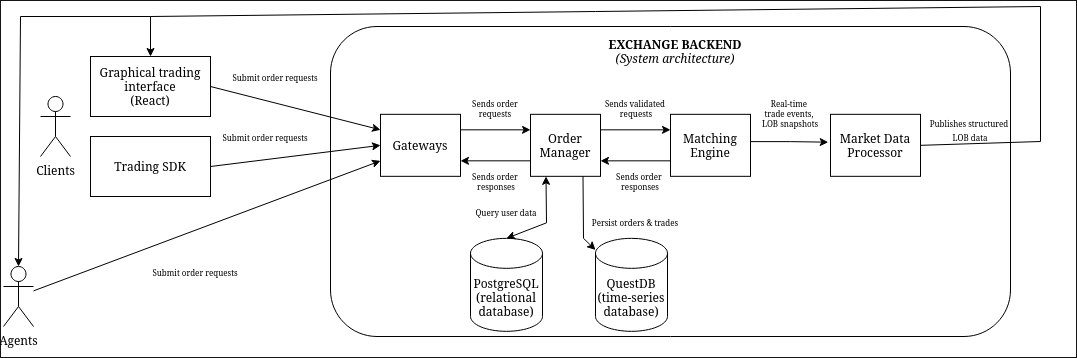
\includegraphics[width=\textwidth]{assets/exch_arch_fig_one.png}
    \caption{High-level system architecture of the exchange backend.}
    \label{fig:design_arch}
\end{figure}

\subsubsection{User Access Layer: SDK \& Graphical Interface}
To provide a seamless experience for both developers and retail-like users, the system exposes two primary interaction points:
\begin{itemize}
    \item \textbf{Trading SDK:} We developed a programmatic interface that abstracts complex networking logic into simple, intuitive commands for order submission and cancellation. This SDK acts as a high-performance bridge between algorithmic strategies and the trading system. To handle real-time execution reports (automated system messages confirming whether an order has been successfully placed, matched, or canceled), the SDK provides an event-driven architecture where users can define custom callback handlers to react to market updates seamlessly.
    \item \textbf{Graphical Trading Interface:} We designed a web-based dashboard inspired by professional brokerages. It serves as the visual analytics layer, rendering real-time market depth and price action. Crucially, this interface also allows users to instantiate their own customized, isolated trading environments. Analogous to "game servers" in multiplayer gaming, each user can create a server that hosts an isolated market with its own distinct set of tickers. This provisioning is orchestrated by the frontend communicating with a backend management service and a deployment manager, ensuring complete sandbox isolation for algorithmic experimentation.
\end{itemize}

\subsubsection{External Facing API Layer: FIX Gateways}
Mirroring real-world exchange architecture, all incoming user requests first hit the gateways to undergo simple message validation before being parsed into internal representations. This layer acts as a protocol translator, handling session management (logins/logouts) and ensuring that incoming requests are syntactically correct. By decoupling connection handling from the core matching logic, the system can scale horizontally to handle high user traffic. For instance, additional gateway instances can be dynamically spawned across different machines when demand spikes, without slowing down the core matching engine.

\subsubsection{Order Validation \& Persistence Layer: Order Manager}
Once a request passes the gateway, it moves to the Order Manager, which serves as the central hub of the backend. It is responsible for semantic validation and data persistence:
\begin{itemize}
    \item \textbf{Semantic Validation:} The manager performs critical checks that the gateway cannot, such as balance checking (verifying sufficient funds for a buy order) and position tracking (verifying sufficient inventory for a sell order).
    \item \textbf{Database Integration:} It interfaces with two distinct databases: a relational database for user profiles, credentials, and account balances; and a time-series database for high-frequency order data. Every order and trade event is persisted to ensure a robust audit trail and to allow for historical simulation replays.
\end{itemize}
After validation, the manager synchronously routes requests to the matching engine and subsequently passes trade confirmations back to the gateway to notify the originating user.

\subsubsection{The Core: Matching\allowbreak Engine \& LOB Data Structures}
This layer is the performance-critical heart of the exchange. The engine receives a validated request, attempts to match it against the opposite side of the Limit Order Book (LOB), generates trade events if a match occurs, and updates the LOB state.
\begin{itemize}
    \item \textbf{Matching Logic:} We utilized the Price-Time Priority algorithm, meaning orders with the best price are matched first, whereas orders at the same price level are executed on a first-come-first-served basis.
    \item \textbf{Data Structure Design:} We designed a theoretically optimal LOB based on algorithmic time complexity. The bid and ask sides are represented as balanced Binary Search Trees (BSTs) to provide $\mathcal{O}(\log N)$ access to price levels. Each price level contains a doubly-linked list of orders to support $\mathcal{O}(1)$ additions at the back of the queue, preserving Price-Time Priority. This is complemented by a hash map that stores iterators to every active order, enabling $\mathcal{O}(1)$ lookups and arbitrary order cancellations without traversing the book.
\end{itemize}

\subsubsection{Distribution Layer: Market Data Processor}
The output from the Matching\allowbreak Engine is raw and high-velocity. The Market Data Processor acts as the system's publisher, transforming core trade events and orderbook updates into accessible formats and broadcasting them to external clients.

To maintain the performance gains achieved by the core engine, the inter-process communication (IPC) channel between the engine and the processor relies on a shared memory mechanism. This architectural choice guarantees that the matching engine is completely decoupled from the unpredictable latency introduced by string serialization and network broadcasts. By strictly delegating these computationally intensive I/O tasks to a separate process, the core engine can continue matching orders unimpeded.

\subsubsection{Simulation Layer: Agents \& Market Regimes}
To provide a realistic and educational venue, the system includes an agent layer that simulates heterogeneous market participants interacting with the gateways just like human clients. We designed three distinct agent-based models to represent different market microstructure participants:
\begin{itemize}
    \item \textbf{Noise Traders:} Operating as a zero-intelligence model, these agents simulate uninformed retail flow. Their order arrivals are governed by a Poisson process, meaning the inter-arrival time $\Delta t$ between consecutive orders follows an exponential distribution:
    \begin{equation}
        f(\Delta t; \lambda) = \lambda e^{-\lambda \Delta t}
    \end{equation}
    where $\lambda$ represents the order intensity (events per second). Order parameters are generated using randomized statistical distributions to provide baseline market activity. Specifically, the side of the order (buy or sell) is determined by a Bernoulli distribution, and the order quantity follows a Pareto distribution, defined by its scale and shape parameters, resulting in heavy-tailed order sizes. The agents are initialized with a configured number of active noise traders and a starting asset inventory.
    \item \textbf{Market Makers:} Implementing the Avellaneda-Stoikov model, these agents provide liquidity by maintaining a ladder of quotes around the spread. They actively manage inventory risk by calculating a reservation price $r$ (the theoretical mid-price adjusted for inventory) and an optimal spread $\delta$:
    \begin{align}
        r &= s - q \gamma \sigma^2 (T - t) \\
        \delta &= \gamma \sigma^2 (T - t) + \frac{2}{\gamma} \ln\left(1 + \frac{\gamma}{k}\right)
    \end{align}
    Here, $s$ is the current market mid-price, $q$ is the agent's inventory, $\gamma$ is the risk aversion parameter, $\sigma^2$ is the asset's price variance, $T - t$ is the time horizon, and $k$ represents the order book density. The optimal bid and ask quotes are then symmetrically placed at $r - \delta/2$ and $r + \delta/2$. Key configurable parameters include the standard order lot size, the inventory risk aversion factor, the order book liquidity density, the operational time horizon, the initial asset holdings, and the total number of market makers deployed.
    \item \textbf{Informed Traders \& Oracle Service:} These agents act on a ``true'' fundamental asset price $V_t$ provided by an external Oracle Service. When instantiated, both the Oracle Service and the simulated markets assume an initial starting fundamental asset price of \$100.0, providing a standardized baseline for subsequent price discovery and stochastic movements. The oracle generates this true price path using a Geometric Brownian Motion (GBM) augmented with Jump Diffusion to simulate sudden exogenous shocks:
    \begin{equation}
        dV_t = \mu V_t dt + \sigma V_t dW_t + V_t dJ_t
    \end{equation}
    where $\mu$ is the drift, $\sigma$ is the volatility, $W_t$ is a standard Wiener process, and $J_t$ represents the jump process, modeled as a compound Poisson process with a specified jump intensity $\lambda$ and a random jump size distribution (defined by a jump mean and standard deviation). This jump term explicitly allows the model to simulate sudden, discontinuous price changes driven by exogenous shocks, such as breaking macroeconomic news or earnings reports. The Oracle service also specifies a broadcast update interval to push these price updates. The Informed Trader continuously polls the order book and the oracle. If it detects a mispricing greater than a threshold $\epsilon$ (e.g., $V_t > P_{ask} + \epsilon$), it executes aggressive snipe orders against lagging market maker quotes using a predefined aggressive order quantity. This introduces adverse selection and efficiently drives the simulated market towards price discovery. The informed trader is also constrained by an initial inventory and a maximum allowed inventory limit.
\end{itemize}

For the purpose of this educational sandbox, the mathematical parameters governing these agents (e.g., the risk aversion $\gamma$, drift $\mu$, and volatility $\sigma$) are initialized via trial and error rather than being strictly calibrated to historical market data. However, they are fully configurable via the frontend interface and deployment configuration files, allowing users to experiment with diverse market regimes such as high-volatility environments or directional trend markets.

\subsection{Implementation}

\begin{figure}[h]
    \centering
    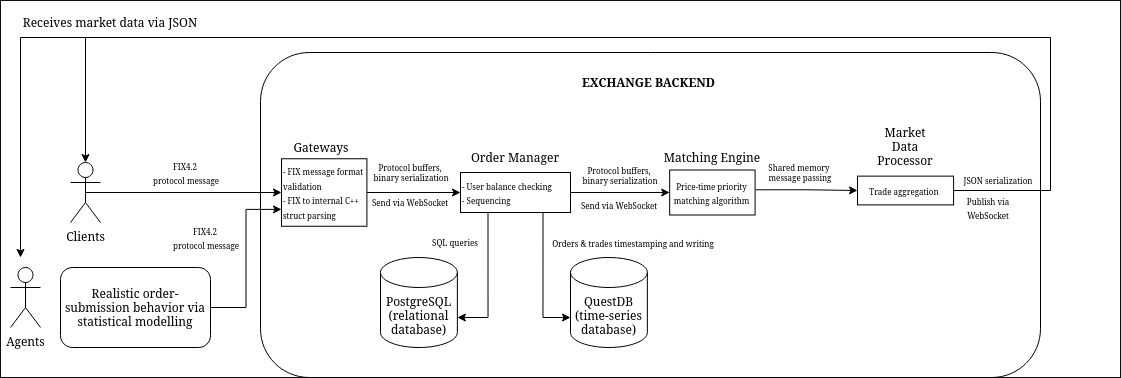
\includegraphics[width=\textwidth]{assets/exch_arch_fig_two.png}
    \caption{Detailed technical implementation of the exchange backend components.}
    \label{fig:impl_arch}
\end{figure}

Our implementation leverages modern C++23, prioritizing low-latency performance and robust type safety. The project uses CMake as its primary build system, facilitating dependency management and modular compilation of the various microservices. External dependencies such as QuickFIX, Boost, Protocol Buffers, and various database clients are integrated directly into the CMake workflow.

To facilitate robust and efficient network communication, we developed a dedicated \texttt{transport} library. For structured message serialization, we utilize Google's Protocol Buffers strictly for internal, inter-service communication (such as routing validated orders from the gateway to the order manager). Their compact binary representation and rapid serialization speeds make them ideal for maintaining a low-latency trading pipeline, whereas text-based formats like JSON are reserved primarily for external communication with the frontend and public APIs. Furthermore, we implemented a custom internal WebSocket library wrapping \texttt{websocketpp}. For architectural convenience, we standardized on WebSockets for almost all internal inter-service communication (with the notable exception of the Matching\allowbreak Engine to Market Data Processor link, which uses a shared-memory ring buffer for ultra-low latency). This same WebSocket infrastructure is seamlessly reused to disseminate real-time market data feeds to the public React frontend.

\subsubsection{User Access Layer: SDK \& Graphical Interface}
The client SDK was developed entirely in C++ to provide developers with a fast and intuitive interface for connecting to the trading system. It exposes a \texttt{FixClient} class that developers can subclass to interact with the market. Key methods include \texttt{submit\_limit\_order}, \texttt{submit\_market\_order}, and \texttt{cancel\_order}, alongside connection management functions. To handle asynchronous execution reports and cancel rejections, the SDK provides virtual callback methods (\texttt{on\_order\_update} and \texttt{on\_order\_cancel\_rejected}) that users can override to implement custom event-driven trading logic.

For the graphical trading interface, we built a responsive single-page application (SPA) using React (\texttt{frontend-v2/src}). The frontend consumes the real-time WebSocket streams from the backend and leverages charting libraries such as \texttt{lightweight-charts} and \texttt{recharts} to dynamically render interactive candlestick charts, price action, and order book depth. Furthermore, the frontend provides a control interface for users to create and manage their isolated market servers. This functionality is achieved by communicating with a backend REST service (\texttt{services/backend\_service}) that orchestrates the provisioning of new environments via a centralized Python deployment script (\texttt{deployment\_server.py}), allowing each user to effortlessly spin up their own independent market "game server."

\begin{figure}[H]
    \centering
    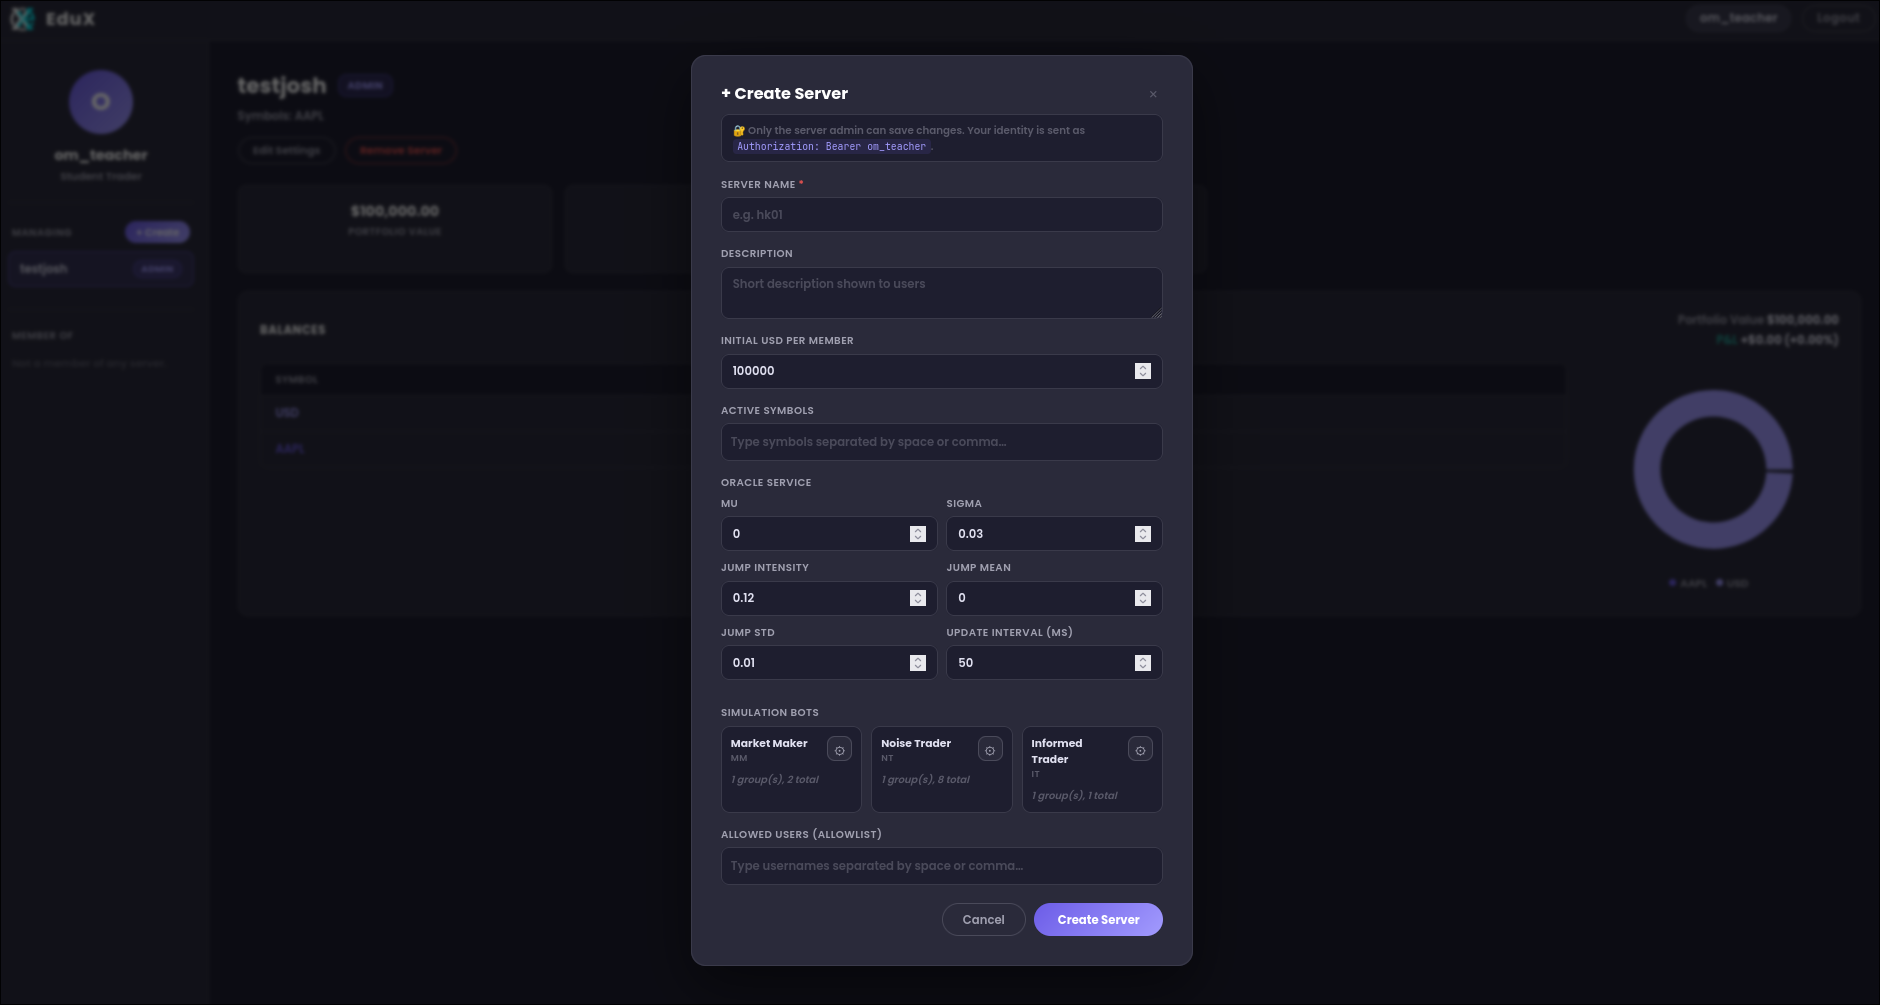
\includegraphics[width=0.85\textwidth]{assets/create_server_step_1_fig.png}

    \vspace{0.5cm}
    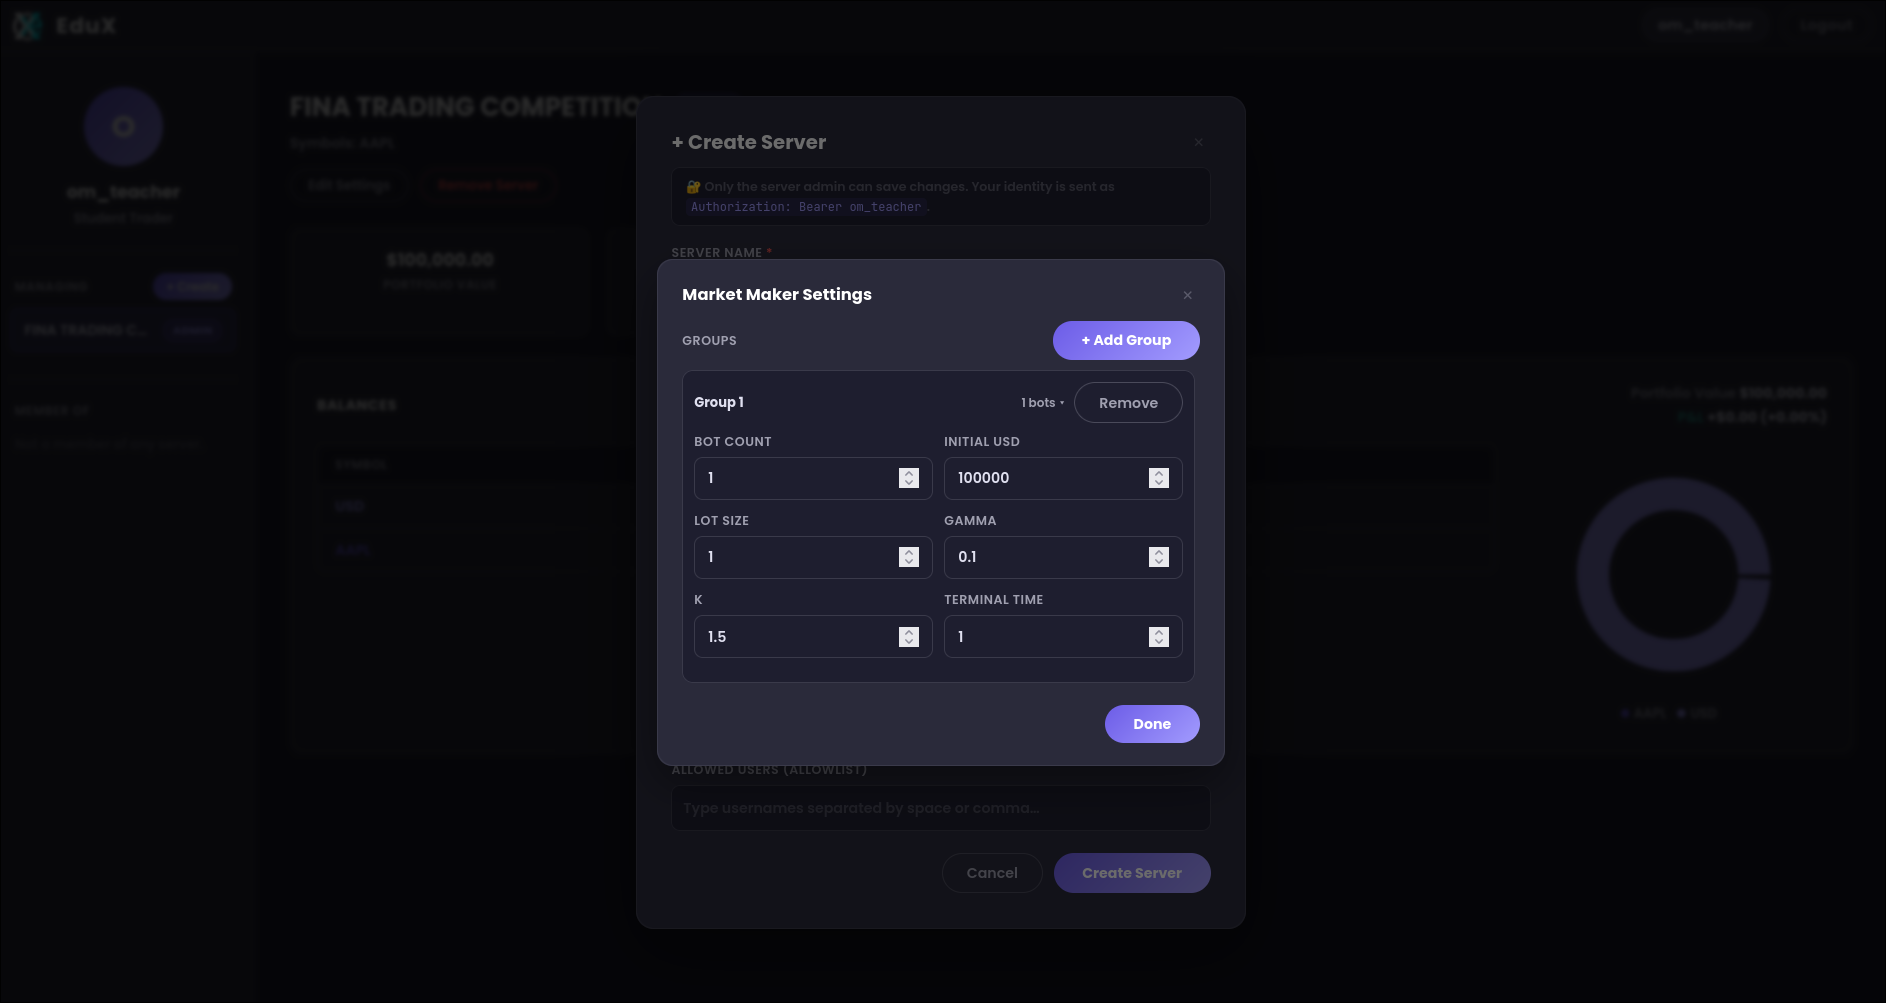
\includegraphics[width=0.85\textwidth]{assets/create_server_step_2_fig.png}
    \caption{Server configuration and deployment interface.}
    \label{fig:ui_create_server}
\end{figure}

\begin{figure}[H]
    \centering
    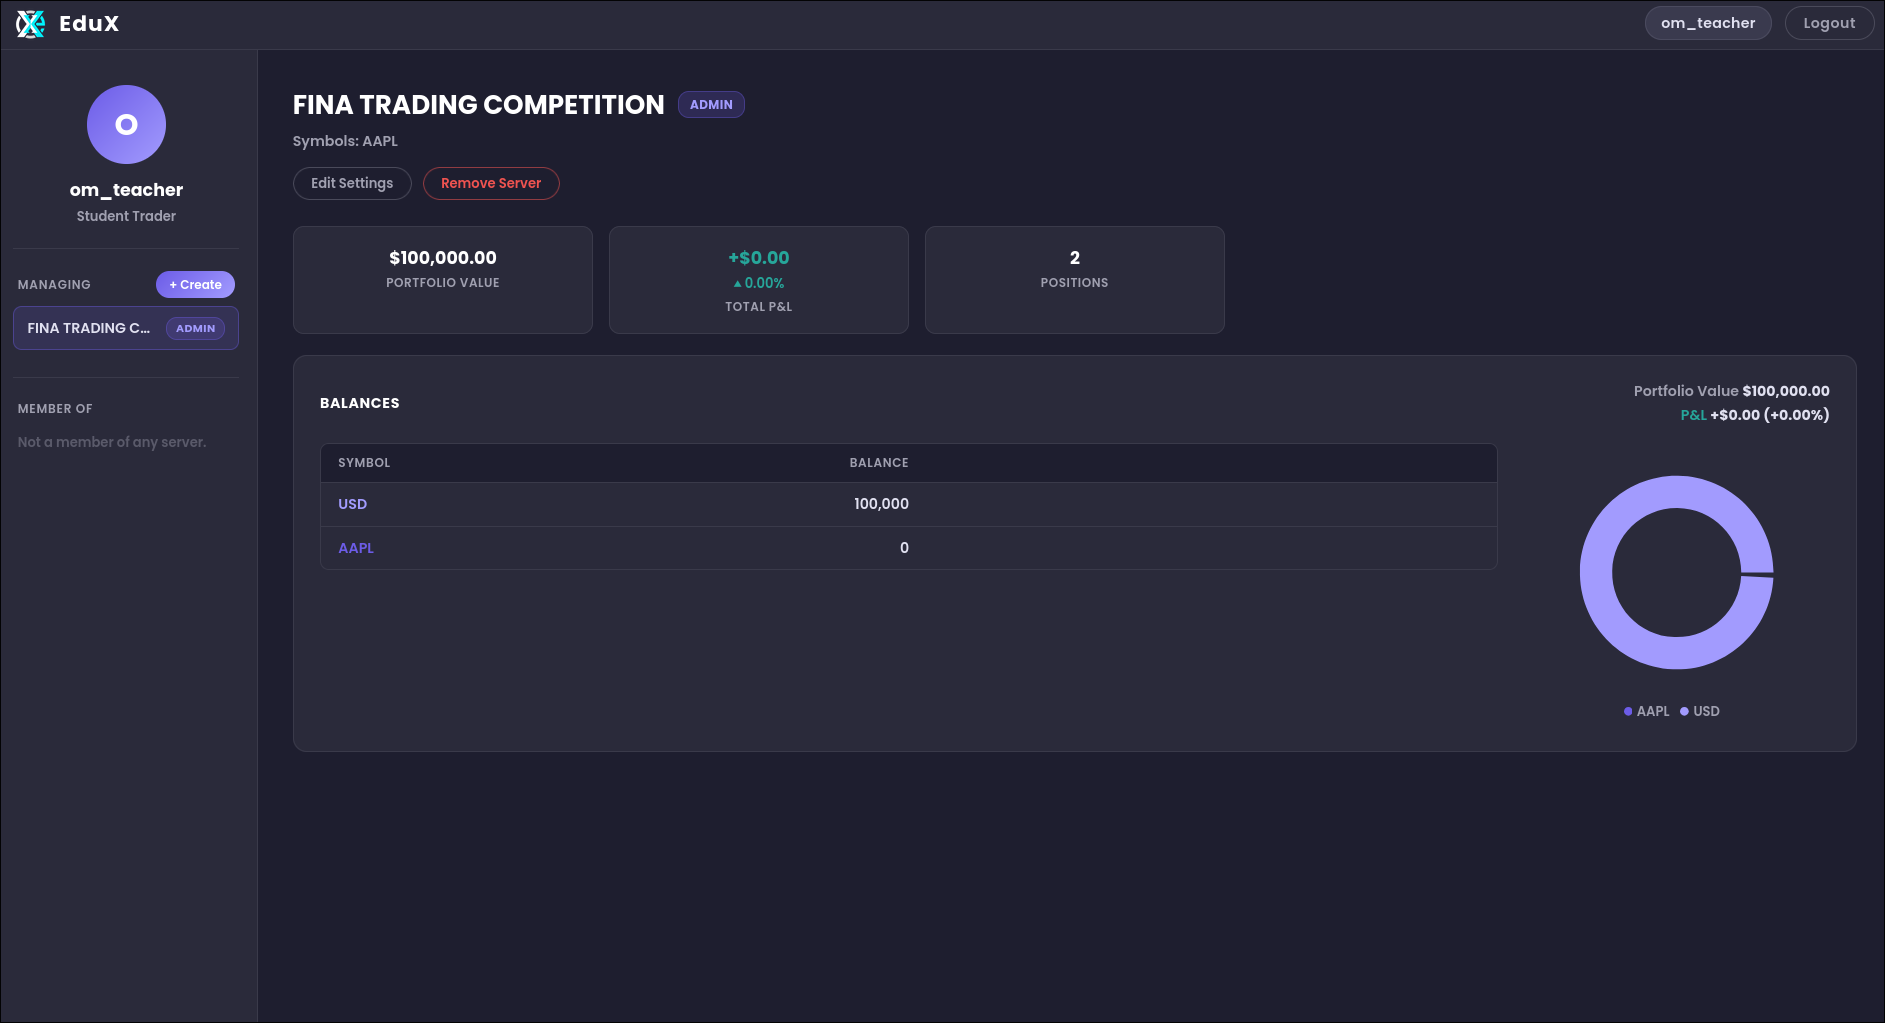
\includegraphics[width=\textwidth]{assets/portfolio_view_fig.png}
    \caption{User portfolio and order management dashboard.}
    \label{fig:ui_portfolio}
\end{figure}

\begin{figure}[H]
    \centering
    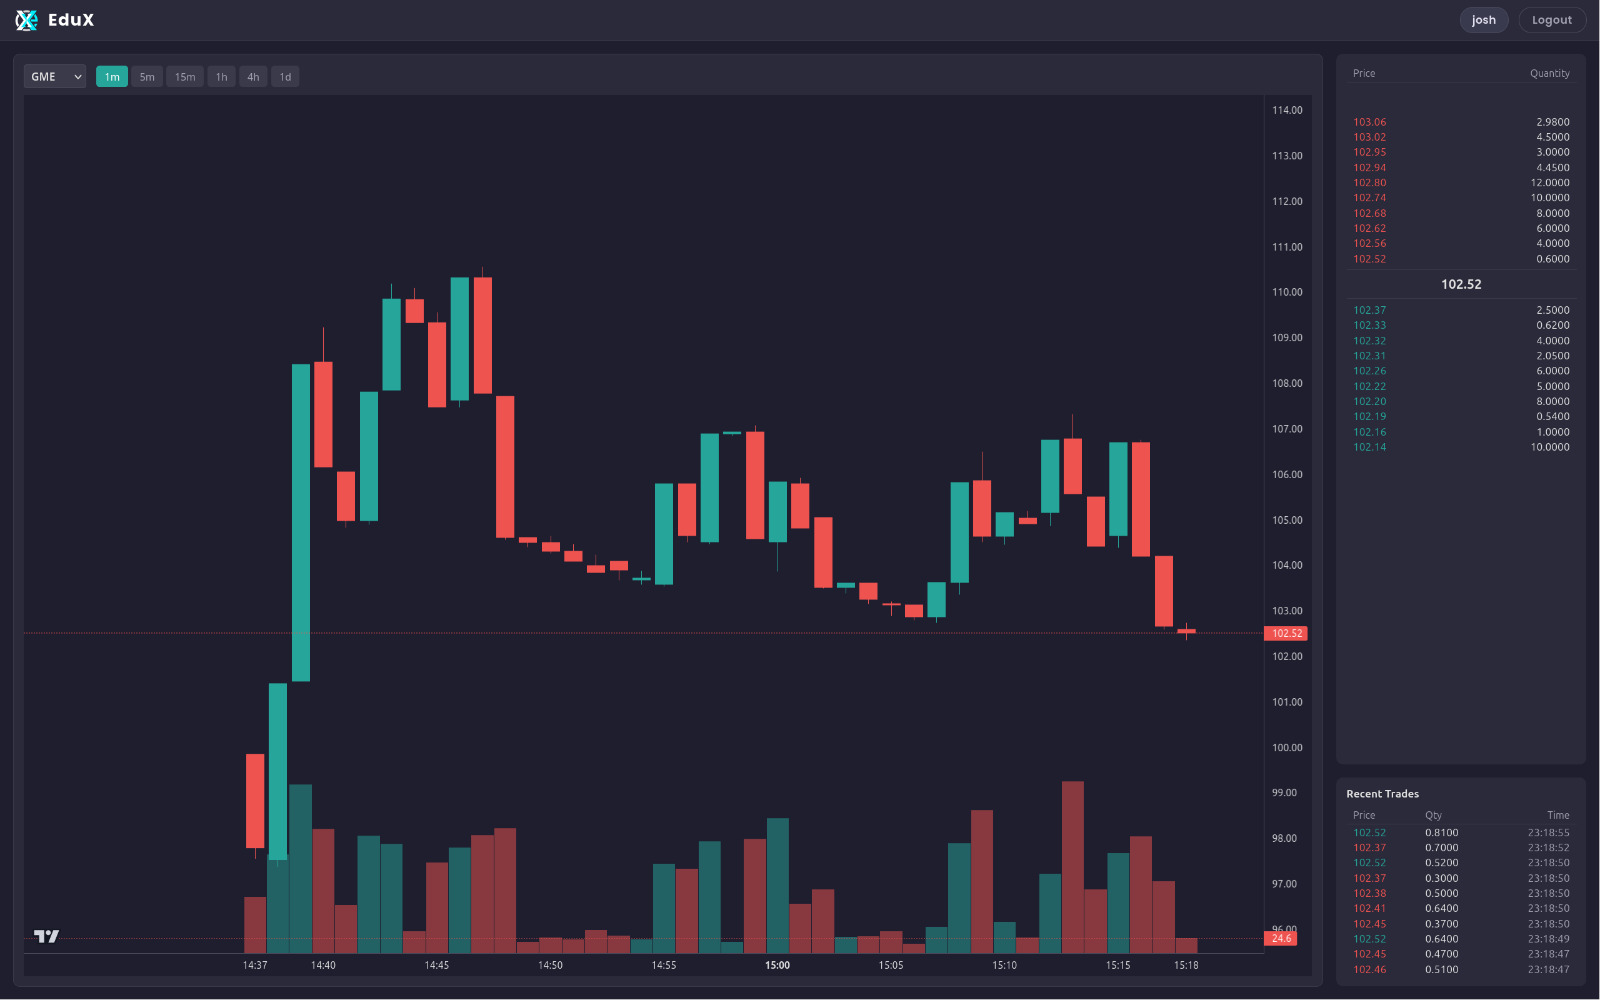
\includegraphics[width=\textwidth]{assets/trading_view_fig.jpeg}
    \caption{Real-time K-line charting and market depth visualization.}
    \label{fig:ui_kline}
\end{figure}

\subsubsection{External Facing API Layer: FIX Gateways}
The FIX Gateway was implemented using the QuickFIX C++ engine. It serves as the external-facing API, parsing incoming FIX protocol messages and translating them into internal data structures. By leveraging QuickFIX, the gateway natively handles session management, message sequencing, and heartbeat mechanisms, ensuring reliable communication with connected clients.

\subsubsection{Order Validation \& Persistence Layer: Order Manager}
The Order Manager acts as a synchronous validator and router. To eliminate race conditions---such as a single user submitting two massive orders simultaneously---the manager processes incoming messages sequentially within a single-threaded event loop. This guarantees that balance constraints and position limits are checked and updated atomically before any request is forwarded to the Matching\allowbreak Engine. To ensure durability without blocking this critical trading path, the persistence layer utilizes a dual-database architecture managed by a custom \texttt{DatabaseClient}.

Relational data, such as account states and user configurations, is managed using a PostgreSQL database accessed via the \texttt{libpqxx} client. Conversely, high-throughput market events and tick data are logged to a QuestDB time-series database. To prevent database I/O from bottlenecking the system, we implemented an \texttt{AsyncWriter} for QuestDB ingestion. This module offloads database writes to a dedicated background thread, buffering operations like order insertions and trade logs into a thread-safe queue. The background thread batches these tasks and flushes them to QuestDB over the Ingress Line Protocol based on configurable thresholds and intervals. While validation and matching engine forwarding are synchronous to ensure correctness, this asynchronous persistence guarantees that database latency does not degrade order processing times.

To illustrate the persistence schema, the time-series definitions for order logs and trade logs in QuestDB are summarized in Tables \ref{tab:questdb_orders} and \ref{tab:questdb_trades}. They are partitioned by day and deduplicated using UPSERT keys, which allows robust, high-throughput historical reconstruction.

\begin{table}[H]
    \begin{minipage}[t]{0.48\textwidth}
        \centering
        \renewcommand{\arraystretch}{1.2}
        \begin{tabular}{|l|l|}
            \hline
            \textbf{Field Name} & \textbf{Data Type} \\
            \hline
            \texttt{ts} & \texttt{TIMESTAMP} \\
            \texttt{order\_id} & \texttt{INT} \\
            \texttt{cl\_order\_id} & \texttt{INT} \\
            \texttt{sender\_comp\_id} & \texttt{VARCHAR} \\
            \texttt{symbol} & \texttt{SYMBOL} \\
            \texttt{side} & \texttt{SYMBOL} \\
            \texttt{order\_qty} & \texttt{INT} \\
            \texttt{filled\_qty} & \texttt{INT} \\
            \texttt{ord\_type} & \texttt{SYMBOL} \\
            \texttt{price} & \texttt{INT} \\
            \texttt{time\_in\_force} & \texttt{SYMBOL} \\
            \texttt{order\_status} & \texttt{SYMBOL} \\
            \hline
        \end{tabular}
        \caption{QuestDB Schema for the Orders Table.}
        \label{tab:questdb_orders}
    \end{minipage}\hfill
    \begin{minipage}[t]{0.48\textwidth}
        \centering
        \renewcommand{\arraystretch}{1.2}
        \begin{tabular}{|l|l|}
            \hline
            \textbf{Field Name} & \textbf{Data Type} \\
            \hline
            \texttt{ts} & \texttt{TIMESTAMP} \\
            \texttt{trade\_id} & \texttt{VARCHAR} \\
            \texttt{price} & \texttt{INT} \\
            \texttt{quantity} & \texttt{INT} \\
            \texttt{symbol} & \texttt{SYMBOL} \\
            \texttt{taker\_id} & \texttt{VARCHAR} \\
            \texttt{maker\_id} & \texttt{VARCHAR} \\
            \texttt{taker\_order\_id} & \texttt{INT} \\
            \texttt{maker\_order\_id} & \texttt{INT} \\
            \texttt{is\_taker\_buyer} & \texttt{BOOLEAN} \\
            \hline
        \end{tabular}
        \caption{QuestDB Schema for the Trades Table.}
        \label{tab:questdb_trades}
    \end{minipage}
\end{table}

\subsubsection{The Core: Matching\allowbreak Engine \& LOB Data Structures}
At the core of the system is the Matching\allowbreak Engine, which manages the Limit Order Book (LOB). The LOB was implemented using C++ standard library node-based containers to achieve the theoretically optimal time complexities. Specifically, \texttt{std::map} maintains the sorted price levels (acting as the BST), \texttt{std::list} maintains the doubly-linked queue of orders at each price level, and \texttt{std::unordered\_map} provides constant-time lookups to the list iterators for instant order cancellations. To communicate executions and market state changes to downstream services, the matching engine writes to a custom Multiple-Producer Single-Consumer (MPSC) lock-free ring buffer. This ring buffer is backed by POSIX shared memory (\texttt{shm\_open} and \texttt{mmap}).

To achieve optimal IPC throughput, the buffer capacity was constrained to a power of two, replacing expensive modulo operations with bitwise AND operations for index wrapping. Additionally, to prevent false sharing, the internal structures incorporate explicit memory alignment and padding (\texttt{alignas(64)} for x86 architectures), ensuring producer and consumer indices reside on separate CPU cache lines. In the edge case where the Market Data Processor (Consumer) falls behind the Matching\allowbreak Engine (Producer), the lock-free ring buffer will report as full. Currently, the engine utilizes a non-blocking \texttt{try\_push} mechanism (as seen in the \texttt{try\_publish} calls); if the buffer is at capacity, new events are dropped to prevent the core matching logic from blocking, emphasizing the need for appropriately sized buffers and fast consumer polling.

Listing \ref{lst:match_order} demonstrates the critical path logic for crossing an incoming order against resting liquidity. The algorithm sequentially walks the best available price levels, decrementing quantities and generating \texttt{Trade} events until the incoming order is either fully filled or the opposing liquidity at marketable prices is exhausted.

\vspace{1em}
\begin{lstlisting}[caption={Limit Order Book Matching Algorithm}, label={lst:match_order}]
void LimitOrderBook::match_order(SideContainer& near_side, SideContainer& far_side, int price,
                                 int remaining_quantity, int order_id, Side side,
                                 std::string_view broker_id) {
    // 1. Iterate through the opposing side of the book as long as we have quantity to fill
    while (!far_side.empty() && remaining_quantity > 0) {
        const auto best_level = (side == Side::bid) ? far_side.begin() : std::prev(far_side.end());
        const auto& best_level_price = best_level->first;

        // 2. Stop matching if the best available price is no longer marketable
        if ((side == Side::bid && price < best_level_price) ||
            (side == Side::ask && price > best_level_price)) {
            break;
        }

        auto& best_level_orders = best_level->second;
        // 3. Execute against orders at the current best price level (Price-Time Priority)
        while (remaining_quantity > 0 && !best_level_orders.empty()) {
            auto& front_order = best_level_orders.front();

            if (const auto order_quantity = front_order.get_quantity();
                remaining_quantity >= order_quantity) {
                // 3a. Incoming order fully consumes the resting order
                remaining_quantity -= order_quantity;
                Trade new_trade = create_trade(order_id, front_order.get_order_id(), broker_id,
                                               front_order.get_trader_id(), ticker,
                                               front_order.get_price(), order_quantity, side);
                trade_publisher->try_publish(new_trade);
                trade_events.emplace(std::move(new_trade));
                order_id_map.erase(best_level_orders.front().get_order_id());
                best_level_orders.pop_front();
            } else {
                // 3b. Resting order partially fills the incoming order
                front_order.fill(remaining_quantity);
                Trade new_trade = create_trade(order_id, front_order.get_order_id(), broker_id,
                                               front_order.get_trader_id(), ticker,
                                               front_order.get_price(), remaining_quantity, side);
                trade_publisher->try_publish(new_trade);
                trade_events.emplace(std::move(new_trade));
                remaining_quantity = 0;
            }
        }

        // 4. Remove the price level if all resting orders are exhausted
        if (best_level_orders.empty()) {
            far_side.erase(best_level_price);
        }
    }

    // 5. If the incoming limit order is not fully filled, add it to the resting book (Maker)
    if (remaining_quantity > 0 && price != MARKET_BID_ORDER_PRICE &&
        price != MARKET_ASK_ORDER_PRICE) {
        order_id_map[order_id] = near_side[price].emplace(near_side[price].end(), order_id, price,
    }
}
\end{lstlisting}

\subsubsection{Distribution Layer: Market Data Processor}
The Market Data Processor (MDP) is implemented as an independent C++ application running a continuous event loop. It instantiates dedicated shared-memory ring buffer consumers for each active trading symbol to process both trades and order book snapshots. During each iteration of its busy-wait loop, the MDP invokes non-blocking \texttt{try\_pop()} operations on these queues to check for new events. When raw trade or order book data structures are detected, the processor utilizes the \texttt{nlohmann::json} library to serialize the binary C++ objects into JSON payloads. Finally, the serialized data is pushed asynchronously to all active subscribers via the WebSocket server, delivering tick-by-tick market updates to the frontend dashboard.

\subsubsection{Simulation Layer: Agents \& Market Regimes}
The simulation layer was constructed utilizing a set of C++ autonomous agent classes (\texttt{NoiseTrader}, \texttt{MarketMaker}, and \texttt{InformedTrader}) that act as independent clients to the exchange. They interface with the system using the same \texttt{FixClient} SDK as human users. Agent actions are driven by background threads, with the \texttt{NoiseTrader} specifically utilizing standard library random number generators (\texttt{std::poisson\_distribution} and \texttt{std::mt19937}) to model the stochastic arrival of retail orders. Meanwhile, the \texttt{InformedTrader} leverages a specialized \texttt{OracleService} process that simulates a fundamental asset price track. The oracle disseminates this continuous price path by broadcasting updates over a dedicated WebSocket channel, which the informed agent consumes to continuously poll for price deviations against the live order book and execute its sniping strategy.

Listing \ref{lst:market_maker} illustrates the core logic for the \texttt{MarketMaker} agent based on the Avellaneda-Stoikov model. The agent dynamically adjusts its reservation price and optimal spread based on real-time market variance and its current inventory risk.

\vspace{1em}
\begin{lstlisting}[caption={Avellaneda-Stoikov Market Maker Strategy}, label={lst:market_maker}]
void MarketMaker::make_market(const std::string& ticker) {
    OrderBookSnapshot ob = m_md_handler->get_latest_orderbook(ticker);
    double mid_price = ob.mid_price() == 0.0 ? 100.0 : ob.mid_price();
    double variance = m_md_handler->calculate_variance(ticker);
    variance = variance == 0.0 ? 0.01 : variance;

    double q = m_fix_client->get_inventory(ticker);
    double q_centered = q - m_initial_inventory;

    auto now = std::chrono::steady_clock::now();
    std::chrono::duration<double> elapsed = now - m_start_time;
    double time_left = std::max(0.0, (m_terminal_time - elapsed.count()) / m_terminal_time);

    // Calculate Reservation Price (r)
    double reservation_price = mid_price - (q_centered * m_gamma * variance * time_left);

    // Calculate Optimal Spread
    double spread = (m_gamma * variance * time_left) +
                    ((2.0 / m_gamma) * std::log(1.0 + (m_gamma / m_k)));

    double optimal_bid = reservation_price - (spread / 2.0);
    double optimal_ask = reservation_price + (spread / 2.0);

    place_quotes(ticker, optimal_bid, optimal_ask, spread);
}
\end{lstlisting}

\subsubsection{Server Setup and Deployment}
To orchestrate the system across a Linux environment, we developed a custom Python-based deployment script. This application functions as a localized control plane that parses TOML configuration files to manage the lifecycle of the various microservices. It automatically validates service names, resolves listening ports, and ensures services are fully ready or safely terminated. By handling the automated startup and teardown of the components—including the FIX Gateway, Order Manager, Matching\allowbreak Engine, and Market Data Processor—the deployment server provides a reliable and reproducible environment for running extensive market simulations.

\subsubsection{Software Engineering Practices}
Throughout the development of this complex system, we adhered to modern C++ software engineering principles and best practices to ensure robustness, maintainability, and performance:

\begin{itemize}
    \item \textbf{Modern C++ Features:} We extensively utilized features from modern C++ standards (C++20/23) to write safer and more expressive code:
    \begin{itemize}
        \item \textbf{\texttt{std::expected}:} Instead of relying heavily on exceptions, which can introduce non-deterministic control flow and performance overhead on the critical path, we used \texttt{std::expected} to return values or error states explicitly. This functional approach makes error handling predictable and type-safe.
        \item \textbf{Monadic Operations (\texttt{std::transform} / \texttt{or\_else}):} We leveraged monadic operations on \texttt{std::expected} and \texttt{std::optional} to chain operations cleanly, avoiding deep nesting of error-checking code and improving readability across our network and service layers.
        \item \textbf{Smart Pointers and RAII:} Resource Acquisition Is Initialization (RAII) and smart pointers (\texttt{std::unique\_ptr}, \texttt{std::shared\_ptr}) were systematically applied across all components. This guaranteed deterministic resource management and strict prevention of memory leaks without relying on manual memory deallocation.
    \end{itemize}
    \item \textbf{Design by Contract \& Assertions:} To catch logic errors early, we adopted the ``Design by Contract'' methodology using the \texttt{boost::contract} library. We liberally applied preconditions, postconditions, and invariant assertions across critical components like the Limit Order Book and Balance Checker. This strict enforcement guarantees that functions only operate when their required state is valid, immediately asserting and failing fast if an invariant (such as an invalid order ID or negative balance) is violated.
    \item \textbf{Design Patterns \& Abstractions:} We employed various structural and creational design patterns to decouple system components. The Factory Pattern (e.g., \texttt{MatchingEngineDependencyFactory}) was utilized to abstract the instantiation of complex dependencies in the Matching\allowbreak Engine and Order Manager. Furthermore, abstract interfaces (e.g., \texttt{InboundServer}, \texttt{Publisher}) and dependency injection were used throughout the architecture. This allowed us to easily swap out implementations (for instance, substituting a real WebSocket server with a mock server during unit testing) without modifying the core business logic.
    \item \textbf{Asynchronous Logging (\texttt{spdlog}):} For observability, we integrated the high-performance \texttt{spdlog} library. To prevent I/O operations from blocking the main execution threads, we configured it with asynchronous sinks (\texttt{spdlog::async\_factory}). The logger also supports configurable log levels via environment variables and includes comprehensive signal handlers (\texttt{SIGINT}, \texttt{SIGTERM}) to ensure all pending logs are safely flushed to disk before a graceful shutdown.
\end{itemize}

\subsection{Testing}
\subsubsection{Test Plan and Methodology}
Our testing strategy encompassed three primary phases: unit testing, integration testing, and performance benchmarking. We initially utilized the Catch2 library for our unit testing framework due to its lightweight and expressive nature. However, as the system's complexity grew, we migrated our test suite to Google Test (gtest). This transition was motivated by Google Test's robust mock-testing facilities (via Google Mock), which allowed us to effectively isolate components using dependency injection.

For unit testing, we verified the core components—including the Client SDK, FIX Gateway, Order Manager, Matching\allowbreak Engine, and Market Data Processor—by simulating diverse order scenarios. A key focus was validating the Price-Time Priority algorithm to ensure orders were filled in the correct sequence. We also performed ``death testing'' using Google Test's \texttt{EXPECT\_DEATH} macro (as seen in our \texttt{limit\_order\_book\_test.cpp}) to verify that the system correctly terminates or asserts when encountering unrecoverable states, such as querying invalid order IDs.

Integration testing focused on the data flow from the Client SDK through the FIX Gateway and Order Manager to ensure that Protobuf serialization and WebSocket communication maintained data integrity. We tested the trade events emitted by the Matching\allowbreak Engine to ensure the end-to-end flow functioned correctly. Regarding stress testing, our high-load evaluations were scoped strictly to individual component benchmarking, such as isolating the Matching\allowbreak Engine's throughput and latency under massive order bursts.

A comprehensive execution matrix of the system's test suite, detailing critical scenarios and expected outcomes across multiple microservices, can be found in Appendix 6.4.

\subsubsection{Locating Logic Errors and Bugs}
Our testing procedures were critical in identifying flaws that were not initially apparent. A significant logic error was discovered regarding a Limit Order Book (LOB) invariant violation. During early testing, the Matching\allowbreak Engine incorrectly attempted to match against the worst ask price rather than the best ask price, as the engine was accessing the end of the ascending price list instead of the beginning. While simple unit tests missed this edge case, running a randomized order submission simulation revealed that ``Ask'' prices were crossing below ``Bid'' prices—a clear violation of market invariants.

This discovery prompted us to adopt the Design by Contract principle, writing more detailed test cases and enforcing preconditions, postconditions, and invariant assertions throughout the Matching\allowbreak Engine code to catch logic bugs early.

\subsection{Evaluation}
\subsubsection{Benchmarking}
We used Google Benchmark across four Git branches. All benchmarks were executed on an AMD Ryzen AI 7 PRO 360 machine with 32 GB RAM running Linux, compiled with GCC utilizing \texttt{-O3} optimization flags. The baseline is the \texttt{benchmark} branch, built in Release mode with assertions and contract checks disabled. The \texttt{lob-dsa}, \texttt{mem-pool}, and \texttt{template} branches are exploratory prototypes for potential future improvements, rather than immediate production defaults.

\noindent\textbf{Matching\allowbreak Engine}

Figure \ref{fig:branch_benchmark_10k} compares the 10,000-order workload across the main latency-sensitive operations. The \texttt{memory-pool} branch is the only variant that consistently improves end-to-end performance over the baseline. Its strongest gain is in no-match order insertion (\texttt{BM\_MatchingEngine\_NewOrderNoMatchBurstLatency}), where latency is reduced from 0.807 ms to 0.434 ms ($\sim$1.86$\times$ faster). It also reduces pure LOB insertion latency from 0.672 ms to 0.257 ms ($\sim$2.61$\times$ faster). This significant speedup occurs because a custom memory pool pre-allocates contiguous blocks of memory at startup, completely bypassing the heavy operating system overhead of dynamic heap allocations (e.g., \texttt{malloc} or \texttt{new}) during rapid bursts of order insertions. In contrast, the \texttt{template-specialization} branch is mostly neutral to slightly slower, and the \texttt{lob-dsa} branch is effectively neutral for these engine-level benchmarks.

\begin{figure}[H]
    \centering
    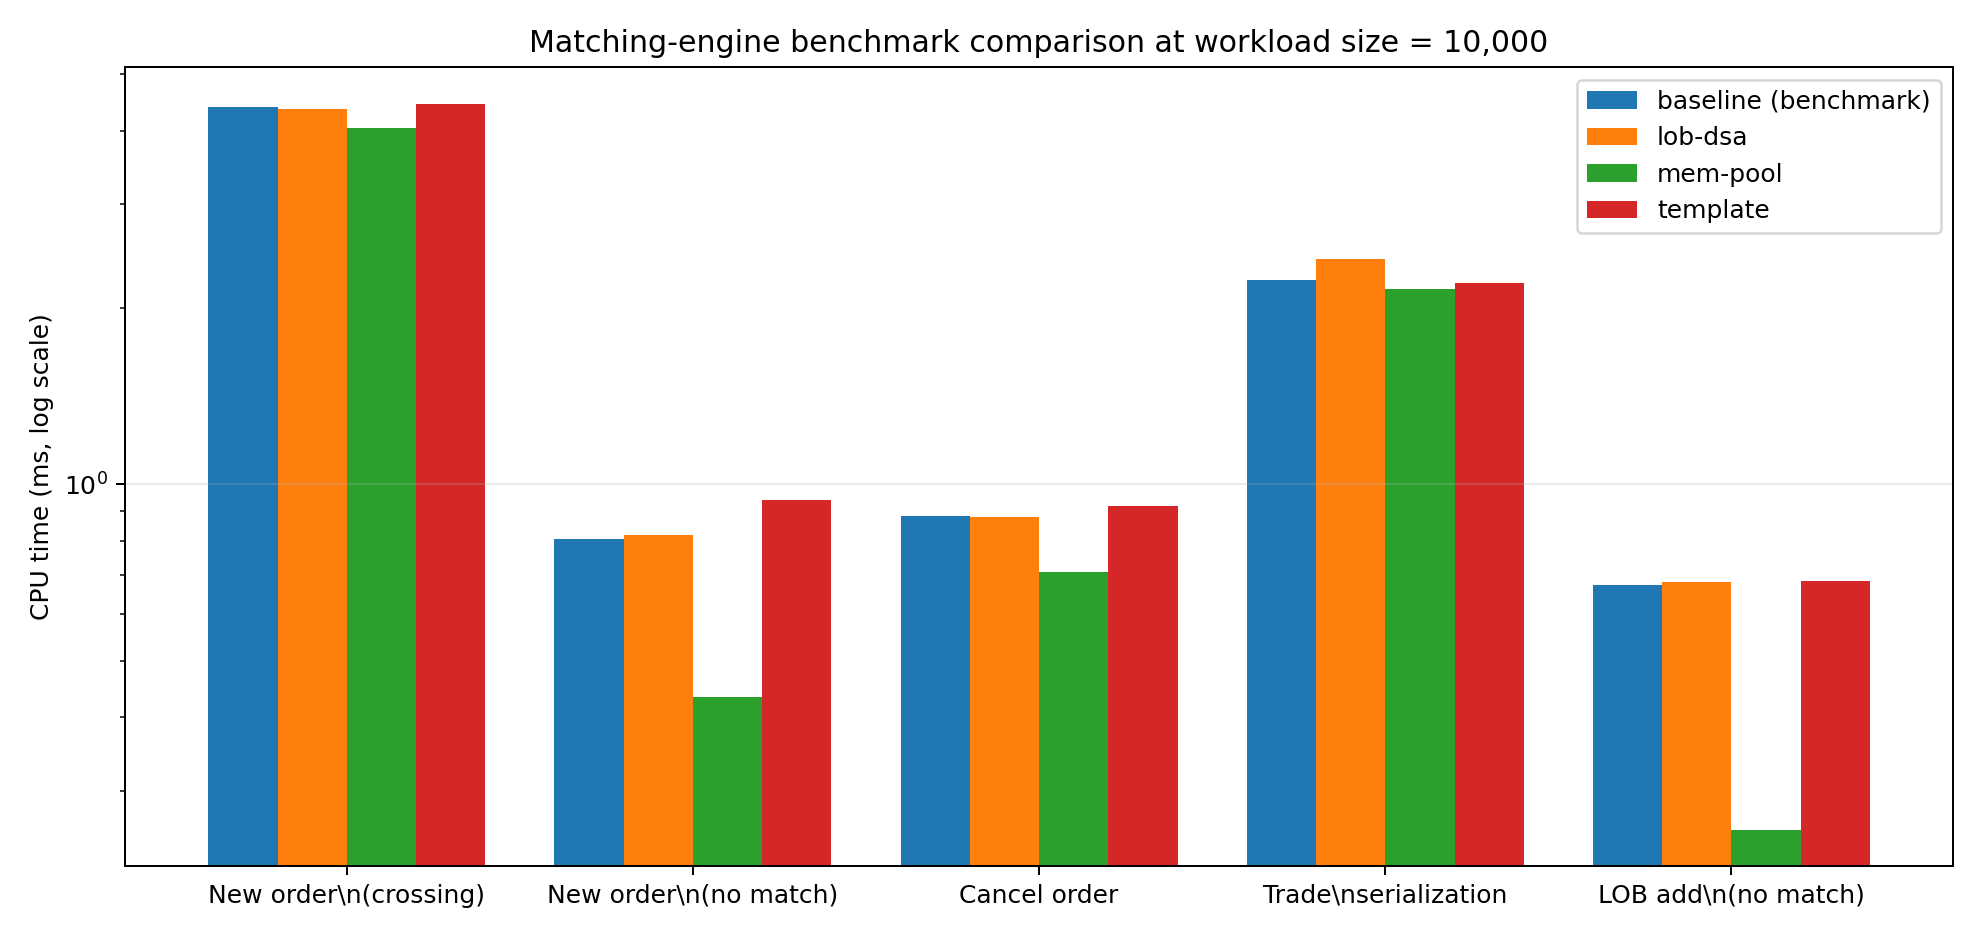
\includegraphics[width=\textwidth]{assets/benchmark_branch_comparison_10k.png}
    \caption{Matching-engine latency comparison across optimization branches at workload size 10,000 (log-scale y-axis).}
    \label{fig:branch_benchmark_10k}
\end{figure}

To isolate the data-structure effect explored in the \texttt{lob-dsa} branch, we also benchmarked a realistic mixed-flow LOB scenario up to 1,000,000 orders (Figure \ref{fig:lob_dsa_scaling}). The vector-based level layout improves large-scale throughput versus the map/list baseline (631.11 ms $\rightarrow$ 353.48 ms at 1,000,000 orders, $\sim$1.79$\times$ faster), while the flat-vector variant degrades sharply at scale due to expensive shifting and maintenance costs under heavy mixed updates. Specifically, inserting or removing an order in the middle of a massive, contiguous flat-vector requires shifting all subsequent elements, meaning the $\mathcal{O}(N)$ algorithmic cost eventually outweighs any hardware benefits gained from CPU cache locality. This result indicates that contiguous storage can outperform node-based structures when the access pattern remains locality-friendly, but only when insertion/cancellation costs are controlled.

\begin{figure}[H]
    \centering
    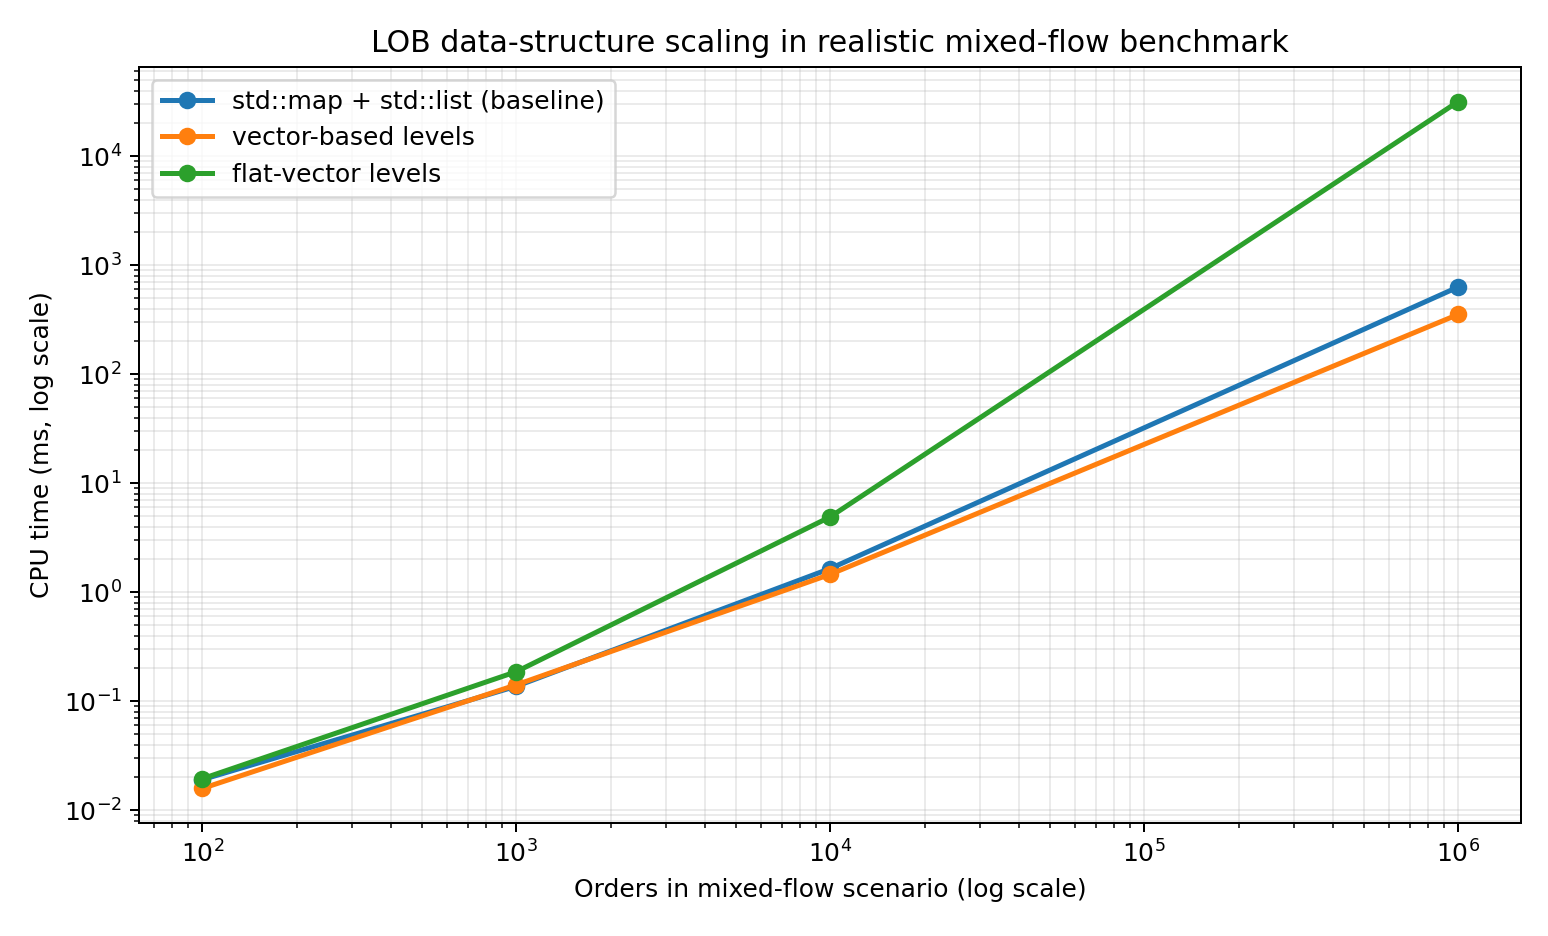
\includegraphics[width=0.9\textwidth]{assets/lob_dsa_structure_scaling.png}
    \caption{LOB data-structure scaling in realistic mixed-flow benchmarks on the \texttt{lob-dsa} branch (log-scale axes).}
    \label{fig:lob_dsa_scaling}
\end{figure}

Table \ref{tab:me_throughput} reports baseline matching-engine throughput for core 10,000-order workloads. Depending on operation type, throughput ranges from 2.28 million to 12.40 million operations per second.

\begin{table}[H]
    \centering
    \renewcommand{\arraystretch}{1.2}
    \begin{tabular}{|l|r|r|}
        \hline
        \textbf{Benchmark (10,000 workload)} & \textbf{Latency (ms)} & \textbf{Throughput (ops/s)} \\
        \hline
        New order (crossing, with matching) & 4.391 & 2,277,274 \\
        New order (no match) & 0.807 & 12,395,537 \\
        Cancel order & 0.882 & 11,333,297 \\
        Trade serialization & 2.233 & 4,478,941 \\
        \hline
    \end{tabular}
    \caption{Baseline matching-engine throughput on the \texttt{benchmark} branch.}
    \label{tab:me_throughput}
\end{table}

These exploratory benchmarks successfully identified improvements to our initial design specification: moving from standard dynamic memory allocation to a custom memory pool is necessary for production-grade throughput, and node-based structures can be effectively replaced by contiguous arrays when carefully managing insertion and deletion costs.

\noindent\textbf{MPSC Lock-Free Ring Buffer}

For the ring buffer component, we measured single-event producer-consumer handoff latency. On the \texttt{benchmark} branch rerun, we observed 771 ns in a single run, with aggregate mean 648.76 ns (manual-time) and 673 ns (CPU-time). This benchmark currently has one configured input amount (one event handoff), shown in Figure \ref{fig:ring_latency_input}.

\begin{figure}[H]
    \centering
    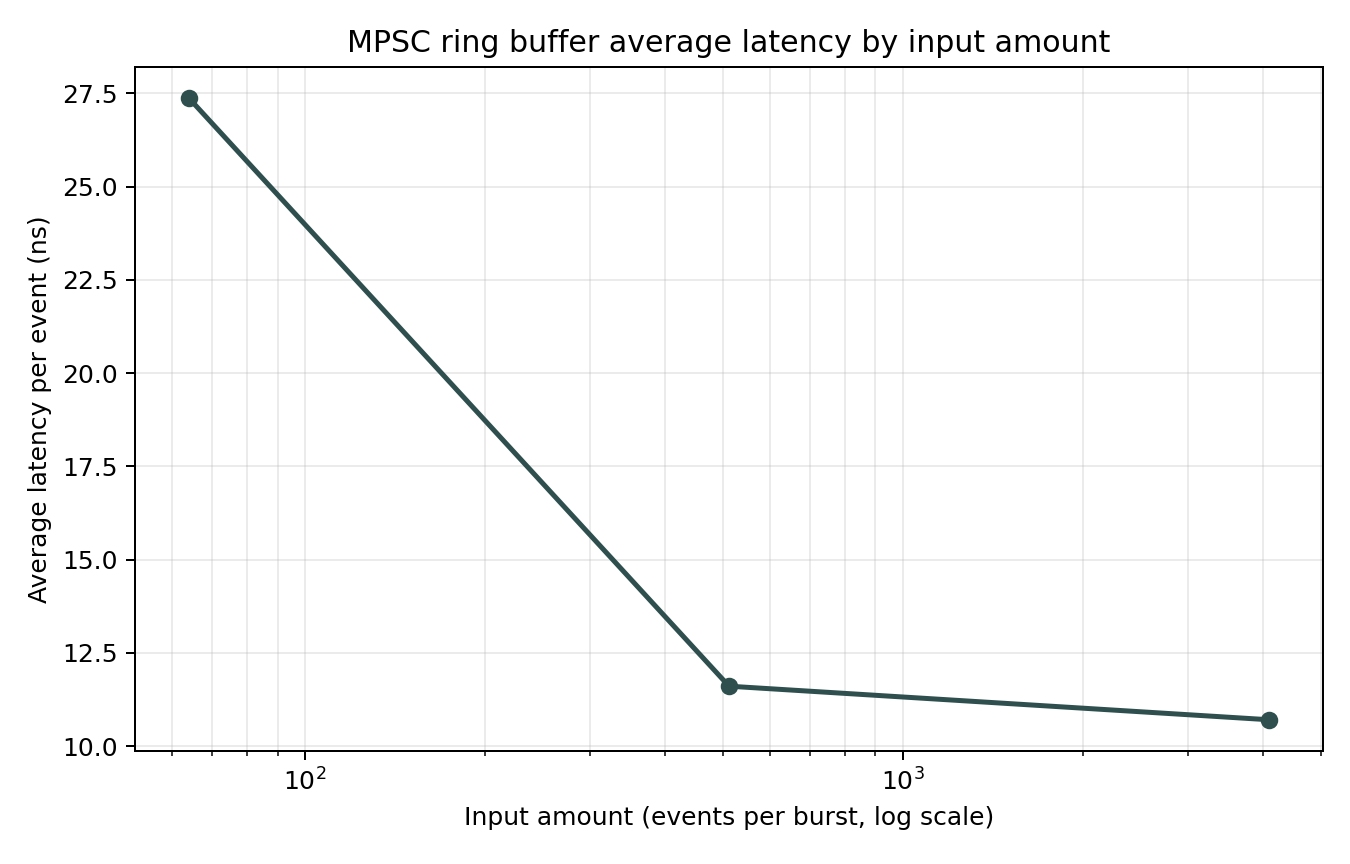
\includegraphics[width=0.7\textwidth]{assets/ring_buffer_latency_by_input.png}
    \caption{MPSC ring buffer average latency by configured input amount.}
    \label{fig:ring_latency_input}
\end{figure}

\noindent\textbf{WebSocket}

For the websocket benchmark on the baseline branch, we measured mean round-trip latency at three payload sizes:
\begin{itemize}
    \item 64 B: 0.03698 ms (\(\sim\)27,042 round-trips/s)
    \item 512 B: 0.04106 ms (\(\sim\)24,353 round-trips/s)
    \item 4096 B: 0.06227 ms (\(\sim\)16,059 round-trips/s)
\end{itemize}
This shows clear latency growth as payload size increases in our local setup.

\begin{figure}[H]
    \centering
    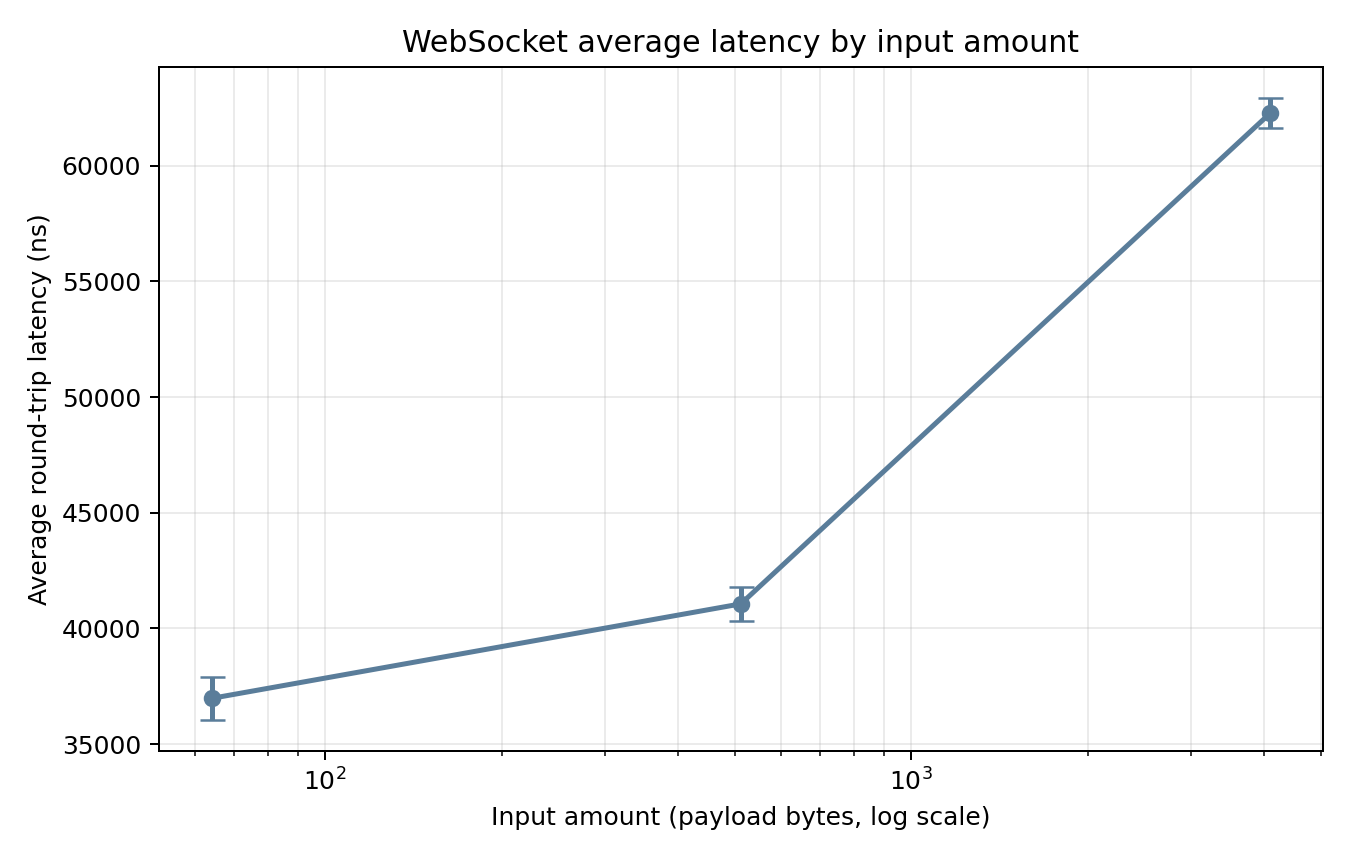
\includegraphics[width=0.85\textwidth]{assets/websocket_latency_by_input.png}
    \caption{WebSocket average round-trip latency by input amount.}
    \label{fig:websocket_latency_input}
\end{figure}

\subsubsection{Simulation Realism}
To evaluate the realism of the simulated market dynamics, we initialize the platform with a baseline configuration across the agent populations. Specifically, the simulation is initialized with 4 Market Makers, 3 Noise Traders, and 1 Informed Trader. The full, detailed list of default parameters for all agent types and the Oracle Service can be found in Appendix \ref{sec:appendix_sim_config}.

Using this baseline configuration, we analyze the resulting order book data to determine whether the simulation exhibits stylized facts commonly observed in real financial markets.


\section{Discussion}

This project successfully delivered a highly modular and functional simulated exchange environment, but it also served as a profound learning experience regarding the extreme engineering constraints of algorithmic trading systems. In this section, we evaluate the deeper reasons behind our successes and shortcomings, and discuss the architectural limitations that would prevent this system from being deployed in a live, high-frequency trading (HFT) production environment.

\subsection{Project Evaluation and Reflections}
We are most confident in our achievement of building a low-latency, strictly correct Limit Order Book and an intuitive C++ SDK. Our success here stems directly from our rigorous adoption of modern C++ paradigms, strict memory management (RAII), and our choice of lock-free data structures. By explicitly isolating the matching engine from network and database I/O, we ensured that the core matching logic—the most critical component of the exchange—could perform optimally without being bottlenecked by external dependencies.

Our approach to the system's distributed architecture also went exceptionally well in terms of logical decoupling. Separating concerns across the FIX Gateway, Order Manager, Matching\allowbreak Engine, and Market Data Processor allowed us to build an elegant ``game server'' provisioning model.

However, our success with realistic market simulation was only partial. While we successfully implemented the mathematical foundations of the Avellaneda-Stoikov market maker and Geometric Brownian Motion, we discovered that generating truly realistic macro-market behaviour requires vastly more sophisticated parameter calibration and multi-agent interaction than a single project timeframe permits. The failure to perfectly replicate real-world volatility was not a flaw in the code, but rather an underestimation of the sheer mathematical complexity involved in modelling human psychological trading factors and macro-economic events.

\subsection{System Limitations}
While our platform serves perfectly as an educational sandbox, several critical factors and architectural shortcuts would discourage its use in a real-world financial institution:

\begin{itemize}
    \item \textbf{Network Latency and IPC Overhead:} We relied heavily on WebSockets for inter-service communication. Even when services are deployed on the same machine, the encapsulation and de-encapsulation overhead of WebSockets is computationally intensive, preventing nanosecond-scale determinism.
    \item \textbf{Cloud Deployment and Load Balancing:} Currently, our deployment orchestration utilizes a Python script locally. We did not leverage separate AWS EC2 instances to test true cross-host microservice deployment or hardware load balancing.
    \item \textbf{Auto-Recovery and Robustness:} The system currently lacks comprehensive auto-recovery mechanisms. In a real exchange, if the Order Manager or Matching\allowbreak Engine crashes, it currently results in dropped messages rather than seamlessly failing over to a hot-standby replica.
    \item \textbf{Concurrency in the Matching\allowbreak Engine:} Our Matching\allowbreak Engine currently processes orders sequentially, which limits the maximum theoretical throughput under massive concurrent load. In industry, this is typically solved by partitioning individual Limit Order Books across independent CPU cores and utilizing the LMAX Disruptor pattern or deterministic state machine replication to achieve massive, lock-free concurrent execution.
    \item \textbf{Database Scalability:} While QuestDB handles our current tick data effectively, scaling to thousands of concurrent users would eventually bottleneck our single-node storage layer due to heavy disk I/O load.
    \item \textbf{Rate Limiting and Flow Control:} The system currently lacks strict rate-limiting at the gateway layer. Without throttling mechanisms, sudden bursts of millions of orders could easily cause buffer overflows or memory exhaustion across the microservice pipeline.
\end{itemize}


\section{Conclusions}

This project successfully culminated in the development of a highly modular, low-latency simulated stock exchange designed for algorithmic trading education. Our major technical accomplishments include the implementation of a Limit Order Book, an intuitive C++ Trading SDK, a dual-database persistence layer, and a modern React-based frontend that orchestrates isolated trading ``game servers.'' Throughout this process, we gained profound insights into the stringent performance and reliability constraints of financial microservices, particularly regarding modern C++ memory management, IPC shared memory, and event-driven architectures.

While we successfully built the core trading pipeline, several problems remain unaddressed for a production-ready system, highlighting exciting avenues for future work. To remedy the system's current limitations, we recommend the following enhancements:

\begin{itemize}
    \item Future iterations should replace WebSockets for internal communication with ultra-low-latency alternatives like Unix domain pipes, UDP multicast, or hardware-accelerated kernel bypassing techniques (e.g., \texttt{AF\_XDP} or DPDK) to eliminate operating system networking stack overhead.
    \item Transitioning from local Python deployment to true CI/CD pipelines deploying across distributed AWS EC2 instances. This should be paired with hardware load balancers and auto-recovery mechanisms (such as distributed consensus and persistent event sourcing) to ensure robust failover.
    \item The matching engine's throughput can be drastically improved by assigning independent CPU threads to different tickers, yielding near-linear scaling without lock contention. Additionally, database sharding should be implemented to partition user and tick data across multiple nodes.
    \item Incorporating more sophisticated mathematical models or AI-driven agents could improve market realism. Furthermore, conducting extensive user testing with volunteer algorithmic traders would provide better data on the SDK's usability and system stability under unpredictable, malicious, or massive loads (e.g., implementing and testing rate-limiting).
\end{itemize}


\section{References}

\begin{thebibliography}{9}

\bibitem{ref1}
M. Aquilina, E. Budish, and P. O’Neill, ``Quantifying the High-Frequency Trading `Arms Race': A New Methodology and Estimates,'' Financial Conduct Authority, Occasional Paper no. 50, 2020. [Online]. Available: \url{https://www.fca.org.uk/publication/occasional-papers/occasional-paper-50.pdf}. [Accessed: Oct. 1, 2025].

\bibitem{ref2}
M. Avellaneda and S. Stoikov, ``High-frequency trading in a limit order book,'' \textit{Quantitative Finance}, vol. 8, no. 3, pp. 217--224, 2008.

\bibitem{ref3}
K. Jain, N. Firoozye, J. Kochems, and P. Treleaven, ``Limit Order Book Simulations: A Review,'' \textit{arXiv preprint arXiv:2402.17359}, Feb. 2024.

\bibitem{ref4}
B. Nigito, ``How to Build an Exchange,'' Jane Street Tech Talks, Jane Street Group, LLC, 2025. [Online]. Available: \url{https://www.janestreet.com/tech-talks/building-an-exchange/}. [Accessed: Oct. 1, 2025].

\bibitem{ref5}
Quod Financial, ``Open Source Multi-Asset Market Simulator: Test Trading Strategies - Quant Replay,'' QuantReplay, 2025. [Online]. Available: \url{https://quantreplay.com/}. [Accessed: Oct. 1, 2025].

\bibitem{ref6}
wkselph, ``How to Build a Fast Limit Order Book,'' \textit{WK's High Frequency Trading Blog}, Feb. 15, 2011. [Online]. Available: \url{https://web.archive.org/web/20110219163448/http://howtohft.wordpress.com/2011/02/15/how-to-build-a-fast-limit-order-book/}. [Accessed: Oct. 1, 2025].

\end{thebibliography}

\newpage
\section{Appendix}

\subsection{Explanation on Limit Order Books}

Electronic markets are governed by centralized Limit Order Books (LOBs), where heterogeneous agents submit, cancel, and execute orders that collectively form price, liquidity, and volatility dynamics. Each Limit Order Book contains a buy side (also called bids) and a sell side (also called asks). If the bid price is greater than or equal to the ask price, the quantity matched will be removed from the LOB. Orders are first sorted by price, then sorted by the earliest time of arrival. This is known as \textit{price-time priority}.

For example, suppose we start with an empty LOB. A trader submits a buy order for one share of APPL at \$100. Since there is no one selling the desired share, this order sits at the ``top'' of the LOB as the best bid. When another trader submits a buy order of one share of APPL at \$99, this bid sits \textit{behind} the \$100 bid due to price-time priority. If another trader then submits a sell order for one APPL share at \$100, there is now a \textit{match} between bid and ask prices, and those orders are filled. All that remains on the LOB is the bid at \$99, becoming the new best bid. If a seller places an ask for \$105, it is clear that no matching is available. This is known as a \textit{bid-ask spread} of \$5. The above example describes limit orders. Another popular type of orders are market orders, which match with the best prices immediately.

This simple mechanism allows for market participants to provide and extract information regarding an asset. For example, a larger bid-ask spread is correlated with lower liquidity, reflecting a riskier trade when entering a position. By aggregating buyer and seller intentions in a central LOB, traders are able to infer the fair price of an asset.

\subsection{Project Planning}
\subsubsection{Distribution of Work \& Gantt Chart}

\begin{table}[H]
\centering
\resizebox{\textwidth}{!}{
\begin{tabular}{|l|c|c|c|c|c|c|c|c|c|c|}
\hline
\multicolumn{11}{|c|}{\textit{G - Gordon \quad J - Josh \quad O - Om}} \\
\hline
\textbf{Task} & \textbf{PIC} & \textbf{Aug} & \textbf{Sep} & \textbf{Oct} & \textbf{Nov} & \textbf{Dec} & \textbf{Jan} & \textbf{Feb} & \textbf{Mar} & \textbf{Apr} \\
\hline
Perform Literature Survey & O & \cellcolor{gray!80} & \cellcolor{gray!80} & & & & & & & \\
\hline
Write Proposal Report & G & \cellcolor{gray!80} & \cellcolor{gray!80} & & & & & & & \\
\hline
Design \& Implement Limit Order Book & J & & \cellcolor{gray!80} & \cellcolor{gray!80} & \cellcolor{gray!80} & & & & & \\
\hline
Design \& Implement Gateway & O & & \cellcolor{gray!80} & \cellcolor{gray!80} & \cellcolor{gray!80} & & & & & \\
\hline
Design \& Implement Order Manager & G & & \cellcolor{gray!80} & \cellcolor{gray!80} & \cellcolor{gray!80} & & & & & \\
\hline
Design \& Implement Market Data Processor & J & & \cellcolor{gray!80} & \cellcolor{gray!80} & \cellcolor{gray!80} & & & & & \\
\hline
Design \& Implement Trade Interface and SDK & J & & \cellcolor{gray!80} & \cellcolor{gray!80} & \cellcolor{gray!80} & & & & & \\
\hline
Test Limit Order Book & G & & & \cellcolor{gray!80} & \cellcolor{gray!80} & & & & & \\
\hline
Test Gateway & O & & & \cellcolor{gray!80} & \cellcolor{gray!80} & & & & & \\
\hline
Test Order Manager & G & & & \cellcolor{gray!80} & \cellcolor{gray!80} & & & & & \\
\hline
Test Market Data Processor & J & & & \cellcolor{gray!80} & \cellcolor{gray!80} & & & & & \\
\hline
Test Trade Interface and SDK & J & & & \cellcolor{gray!80} & \cellcolor{gray!80} & & & & & \\
\hline
Design \& Implement System Architecture \& Infrastructure & G & & & & \cellcolor{gray!80} & \cellcolor{gray!80} & \cellcolor{gray!80} & & & \\
\hline
Design \& Implement Traffic \& Connection Management & O & & & & \cellcolor{gray!80} & \cellcolor{gray!80} & \cellcolor{gray!80} & & & \\
\hline
Test System Architecture \& Infrastructure & G & & & & & \cellcolor{gray!80} & \cellcolor{gray!80} & & & \\
\hline
Test Traffic \& Connection Management & O & & & & & \cellcolor{gray!80} & \cellcolor{gray!80} & & & \\
\hline
Design, Implement \& Test Market Simulation Models & O & & & & & \cellcolor{gray!80} & \cellcolor{gray!80} & \cellcolor{gray!80} & \cellcolor{gray!80} & \\
\hline
Write Progress Report & J & & & & & & \cellcolor{gray!80} & & & \\
\hline
Write Final Report & G & & & & & & & & & \cellcolor{gray!80} \\
\hline
Record Presentation Video & J & & & & & & & & & \cellcolor{gray!80} \\
\hline
Prepare Presentation Deck & O & & & & & & & & & \cellcolor{gray!80} \\
\hline
\end{tabular}
}
\caption{Project Timeline and Task Distribution}
\end{table}

\subsection{Required hardware \& software}
\subsubsection{Hardware}

\begin{itemize}
    \item Linux x86\_64 machine (Fedora 43, kernel 6.19.8)
    \item CPU: AMD Ryzen 5 6600H (6 cores / 12 threads, up to 4.57 GHz)
    \item Memory: 32 GiB RAM
\end{itemize}

\subsubsection{Software}

\begin{itemize}
    \item React and JavaScript for frontend development
    \item C++23 as core programming language
    \item PostgreSQL (locally hosted)
    \item QuestDB (locally hosted)
\end{itemize}

\subsection{Comprehensive Test Cases}
Table \ref{tab:comprehensive_test_cases} provides a comprehensive matrix of test cases extracted from the Google Test suites across multiple backend services (Matching\allowbreak Engine, Order Manager, and Backend\allowbreak Service) and Catch2 suites for common libraries. While we initially used Catch2 for its lightweight nature and continued to use it for our base libraries, we migrated to Google Test for our complex backend services to leverage its robust mocking framework. This matrix serves as evidence of the rigorous execution testing and validation of system invariants.

\begingroup
\renewcommand{\arraystretch}{1.2}
\small
\begin{longtable}{|>{\raggedright\arraybackslash}p{2.8cm}|>{\raggedright\arraybackslash}p{2.2cm}|>{\raggedright\arraybackslash}p{3.2cm}|>{\raggedright\arraybackslash}p{2.3cm}|>{\raggedright\arraybackslash}p{2.3cm}|>{\raggedright\arraybackslash}p{1.2cm}|}
\caption{Comprehensive execution matrix of test cases across backend services and common libraries.}\label{tab:comprehensive_test_cases}\\
\hline
\textbf{Test Name} & \textbf{Component} & \textbf{Scenario/\allowbreak Description} & \textbf{Expected\allowbreak Result} & \textbf{Actual\allowbreak Result} & \textbf{Pass\allowbreak/Fail} \\
\hline
\endfirsthead
\caption*{Table \thetable: Comprehensive execution matrix of test cases across backend services and common libraries (continued)}\\
\hline
\textbf{Test Name} & \textbf{Component} & \textbf{Scenario/\allowbreak Description} & \textbf{Expected\allowbreak Result} & \textbf{Actual\allowbreak Result} & \textbf{Pass\allowbreak/Fail} \\
\hline
\endhead
\hline \multicolumn{6}{r}{\textit{Continued on next page}} \\
\endfoot
\hline
\endlastfoot
        \texttt{Match\allowbreak Multiple\allowbreak Standing\allowbreak Bid\allowbreak Orders} & Matching\allowbreak Engine & Aggressive ask order matches against multiple limit buy orders at the same price level. & Orders matched strictly in arrival time sequence (Price-Time Priority). & Matches generated in correct temporal order. & Pass \\
        \texttt{Completely\allowbreak Fill\allowbreak Standing\allowbreak Bid\allowbreak Order} & Matching\allowbreak Engine & Aggressive ask order crosses and exactly fills resting bid order. & Single trade executed; resting bid completely removed from LOB. & Trade generated; LOB updated correctly. & Pass \\
        \texttt{Partially\allowbreak Fill\allowbreak Market\allowbreak Ask} & Matching\allowbreak Engine & Market ask order partially filled by available resting bids. & Trade generated for available quantity; market order fully consumed. & Trade generated; remainder of book unmodified. & Pass \\
        \texttt{Add\allowbreak Market\allowbreak Order\allowbreak To\allowbreak Empty\allowbreak Book} & Matching\allowbreak Engine & Market order submitted when no opposing liquidity exists. & Order rejected or stored temporarily (depending on rule) with zero fill. & Handled gracefully without crash. & Pass \\
        \texttt{Cancel\allowbreak Invalid\allowbreak Order} & Matching\allowbreak Engine & \texttt{Cancel\allowbreak Order\allowbreak Death\allowbreak Test} attempts to cancel a non-existent Order ID. & Contract assertion failure / death test triggered gracefully. & Process terminated via assertion as expected. & Pass \\
        \texttt{Get\allowbreak Invalid\allowbreak Order\allowbreak I\allowbreak D} & Matching\allowbreak Engine & \texttt{Getters\allowbreak Death\allowbreak Test} queries a non-existent Order ID. & Contract assertion failure. & Process terminated via assertion. & Pass \\
        \hline
        \texttt{Insufficient\allowbreak Balance} & Order Manager & \texttt{Has\allowbreak Sufficient\allowbreak Balance\allowbreak Test} checks if a trade exceeds current broker balance. & Validator returns false; order rejected before routing. & Returned false; balance remains unchanged. & Pass \\
        \texttt{Decrement\allowbreak Below\allowbreak Zero} & Order Manager & \texttt{Update\allowbreak Balance\allowbreak Death\allowbreak Test} attempts to decrement balance below 0. & Contract assertion failure / death test triggered. & Process terminated via assertion. & Pass \\
        \texttt{Invalid\allowbreak Cancel\allowbreak Request} & Order Manager & Validation of an improperly formed cancel request payload. & Validator flags payload as malformed. & Rejected prior to matching engine. & Pass \\
        \texttt{Valid\allowbreak Market\allowbreak Bid} & Order Manager & Validation of a properly formed market bid payload. & Passes semantic checks; forwards to engine. & Successfully forwarded to Matching\allowbreak Engine. & Pass \\
        \texttt{Forward\allowbreak And\allowbreak Reply\allowbreak Fails} & Order Manager & \texttt{Forward\allowbreak And\allowbreak Reply\allowbreak Test} checks behavior when Matching\allowbreak Engine connection drops. & Order Manager gracefully handles socket failure and replies with rejection. & Rejection report sent to user. & Pass \\
        \hline
        \texttt{Login\allowbreak Wrong\allowbreak Password} & Backend\allowbreak Service & User attempts login with incorrect credentials. & Service returns 401 Unauthorized. & HTTP 401 returned. & Pass \\
        \texttt{Signup\allowbreak Duplicate\allowbreak User} & Backend\allowbreak Service & Registration attempt with an existing email/username. & Service returns 409 Conflict or 400 Bad Request. & Correct error code returned. & Pass \\
        \hline
        \texttt{Basic\allowbreak Enqueue\allowbreak Dequeue} & Thread Safe Queue (Catch2) & Single-threaded enqueue and dequeue operations. & Elements are enqueued and dequeued in FIFO order. & Operations succeed and order is preserved. & Pass \\
        \texttt{Multithreaded\allowbreak Producer\allowbreak Consumer\allowbreak Correctness} & Thread Safe Queue (Catch2) & Multiple producers and consumers operating concurrently. & All elements are processed without data races or deadlocks. & Data integrity maintained across threads. & Pass \\
        \texttt{insert\_ \allowbreak order succeeds and row is queryable} & Database Client (Catch2) & Inserting a new order record into the database. & Order is successfully inserted and can be retrieved. & Record stored and queried successfully. & Pass \\
        \texttt{concurrent insert\_ \allowbreak order from multiple clients} & Database Client (Catch2) & High-concurrency insertions from multiple threads. & All orders are inserted accurately without dropped transactions. & Database handles concurrent writes correctly. & Pass \\
        \texttt{M\allowbreak P\allowbreak S\allowbreak C \allowbreak Producer/\allowbreak Consumer} & Lock-free Queue (Catch2) & Single producer and consumer operating over a lock-free queue. & Messages are safely passed without locks. & High-throughput message passing achieved. & Pass \\
        \texttt{Client \allowbreak Server \allowbreak Ping \allowbreak Pong} & Network/\allowbreak WebSocket (Catch2) & Bi-directional message echoing between client and server. & Messages are received intact and in order. & Successful real-time communication. & Pass \\
        \texttt{Two \allowbreak Client \allowbreak One \allowbreak Server} & Network/\allowbreak WebSocket (Catch2) & Multiple clients connecting and communicating with a single server concurrently. & Server correctly identifies and routes messages to respective clients. & Multiplexed communication successful. & Pass \\
        \hline
    \end{longtable}
\endgroup


\subsection{Simulation Default Configuration}
\label{sec:appendix_sim_config}
The following tables outline the complete default configuration values used to initialize the simulation platform's agents and the Oracle Service.

\begin{table}[H]
    \centering
    \renewcommand{\arraystretch}{1.2}
    \begin{tabular}{|l|l|l|}
        \hline
        \textbf{Component} & \textbf{Parameter Name} & \textbf{Default Value} \\
        \hline
        Noise Trader & \texttt{num\_noise\_traders} & 3 \\
        & \texttt{lambda\_eps} & 0.6 \\
        & \texttt{bernoulli} & 0.5 \\
        & \texttt{pareto\_scale} & 0.5 \\
        & \texttt{pareto\_shape} & 4.0 \\
        & \texttt{initial\_inventory} & 20.0 \\
        \hline
        Market Maker & \texttt{num\_market\_makers} & 4 \\
        & \texttt{lot\_size} & 1.0 \\
        & \texttt{gamma} & 0.6 \\
        & \texttt{k} & 8.0 \\
        & \texttt{terminal\_time} & 30.0 \\
        & \texttt{initial\_inventory} & 300.0 \\
        \hline
        Informed Trader & \texttt{num\_informed\_traders} & 1 \\
        & \texttt{initial\_inventory} & 100.0 \\
        & \texttt{epsilon} & 0.05 \\
        & \texttt{trade\_qty} & 10.0 \\
        & \texttt{max\_inventory} & 1000.0 \\
        \hline
        Oracle Service & \texttt{mu} & 0.0 \\
        & \texttt{sigma} & 0.003 \\
        & \texttt{jump\_intensity} & 0.06 \\
        & \texttt{jump\_mean} & 0.0 \\
        & \texttt{jump\_std} & 0.01 \\
        & \texttt{update\_interval\_ms} & 60000 \\
        \hline
    \end{tabular}
    \caption{Complete default configuration parameters for the simulation components.}
    \label{tab:full_sim_configs}
\end{table}

\end{document}
